\documentclass[UTF8]{ctexart}
\usepackage{amsmath}
\usepackage{amssymb}
\usepackage{bm}
\usepackage{fancyhdr}
\usepackage{booktabs}
\usepackage{breqn}
\usepackage{color}
\usepackage{enumitem}
\usepackage{float}
\usepackage{graphicx}
\usepackage{multirow}
\usepackage{hyperref}
\usepackage{indentfirst}
\usepackage{multicol}
\usepackage{ntheorem}
\usepackage{subfigure}
\usepackage{txfonts}
\usepackage{algorithm}
\usepackage{algorithmic}
\setlength{\parindent}{2em}
\usepackage{IEEEtrantools}
\usepackage{geometry}
\graphicspath{{figs/}}
\floatname{algorithm}{算法}  
\renewcommand{\algorithmicrequire}{\textbf{输入:}}  
\renewcommand{\algorithmicensure}{\textbf{输出:}} 
\date{2021年4月}
\author{
	敖睿成\quad 吴熙楠 \quad 高玮伯 \quad 杨轩}
\title{
	\heiti{传染病模型与疫苗接种}
}

\hypersetup{
	colorlinks=true,
	linkcolor=black
}
\begin{document}
	\maketitle
	\newtheorem{definition}{定义}[subsection]
	\newtheorem{function}{公式}[subsection]
	\newtheorem{summary}{小结}[subsection]
	\newtheorem{deduction}{推论}[subsection]
	\newtheorem{property}{性质}[subsection]
	\newtheorem{theo}{定理}[subsection]
	\newtheorem{step}{步骤}[subsection]
	\newtheorem{remark}{注记}[subsection]
	\newtheorem{proof}{证明}[subsection]
	\newenvironment{Theorem}[1][]{\par\noindent\textbf{定理}(#1)\quad}{\par}
	\newcommand{\rbra}[1]{\left( #1 \right)}
	\newcommand{\sbra}[1]{\left[ #1 \right]}
	\newcommand{\cbra}[1]{\left\{ #1 \right\}}
	\newcommand{\pbra}[1]{\left< #1 \right>}
	\newcommand{\abs}[1]{\left| #1 \right|}
	\newcommand{\fs}[2]{\displaystyle\frac{#1}{#2}}
	
	\newenvironment{myproof}{{\color{blue}证:}}
	
	\newenvironment{partlist}[1][]
	{\begin{enumerate}[itemsep=0pt, label=(\arabic*), wide, labelindent=\parindent, listparindent=\parindent, #1]}
		{\end{enumerate}}
	
	\renewcommand{\contentsname}{目录} %将content转为目录
	\tableofcontents
	\newpage
	\renewcommand{\abstractname}{\large 摘要\\}
	\begin{abstract}
    在去年新型冠状病毒引发疫情,并在世界范围内快速传播,在过去的一年内,肺炎感染了数以千万计的人,虽然现在世界上多个国家已经开启了对国民的疫苗接种计划,但距离完全控制疫情仍有很长的路,同时如何分配疫苗也是一大难题。
    
	本文将对此次疫情建模,首先通过经典的SIR模型与SEIR模型对感染数据进行拟合,然后更有针对性地用时滞模型进行建模,之后是基于随机过程进行建模,然后研究传染病模型中的最优控制问题,最后引入网络模型分析了传染病的传播过程以及对疫苗接种问题进行了一些讨论。

    \end{abstract}
	\section{绪论}
	传染病是人类极具杀伤力的敌人,尽管人类在其他领域取得了重大成就,如LIGO探测到双黑洞并和产生的引力波,我们仍然没有根除大多数疫苗可预防的传染病,如埃博拉病毒、寨卡病毒和SARS,还有最新的新冠病毒,不断从动物中出现向人类传播,这些传染病除了疫苗接种预防以外并没有其他行之有效的解决办法,因此了解和建立传染病传播模型以及确立疫苗分配接种方案成了目前的重要任务,我们本文的目的也是通过从最基础的SIR和SEIR模型出发,建立传染病数学模型,并进行数值检验,以及讨论部分传染病传播以及疫苗接种以及最佳分配问题,从而对于本次还未过去的新冠疫情有更好地理解与反思。
	\par 在本文的第二节中,我们对最基本的SIR模型进行了理论分析建立方程;在第三节中我们对SIR模型进行了武汉数据测验以及讨论了其数值敏感度;在第四节中我们引入已感染处于潜伏期的人群,建立了更为完善的SEIR模型,并讨论其参数以及进行数值测验;在第五节中,我们考虑了疫情传播过程的信息延迟现象,增加出现症状但未被确诊的人群,引入了时滞,并对时滞模型进行了理论与数值检验;在第六节中我们进行了基于随机过程的传染病建模,预测了模型中存在的关于传染病传播的特殊情况;第七节中我们讨论了传染病模型中的最优控制问题,同时在SIR模型下简单讨论了疫苗分发的优化问题;第八节我们建立了一个传染病传播的网络模型,将空间扩散引入传染病传播模型;第九节中我们考虑了在网络中引入疫苗接种节点,简单讨论了需要控制传染病传播的疫苗接种阈值;最后本文以第十节中对本文的总结与展望中结束。	
	    \section{模型建立的理论分析}
			\subsection{方程建立}
				首先将总体分为三类人群,建立最基本的SIR模型(\emph{suscepicble, infected, restored}),假设康复人群不会再被感染,即$S\rightarrow I\rightarrow R$是单向的,同时,总人数也不变,在这种情况下,我们考虑这样一种分布:对于一个独立的个体,其保持在原有状态的时间长$t$满足概率分布$F(t)$,这样,令$G(t)=1-F(t)$,则$G(t)$即为在时间$t$之后仍然在该状态的概率.现在再作出假设:对于$I$和$S$两个人群,他们之间的个体接触可能性不存在差异,即把同一人群的每个人看作相同,接触概率只与$I(t)S(t)$成比例的一个值,同时接触者受到感染的几率是定值.这样,对于$\tau>0,\tau<t$,在$\tau$时间受到感染,并且在$t$时候仍然是感染者的人数为\[\lambda I(\tau)S(\tau)G(t-\tau),\]从而得到第一个方程:
				\begin{eqnarray*} \label{First}
					I(t)&=& I_0(t)+\int_{0}^{t}\lambda I(\tau)S(\tau)G(t-\tau)d\tau,\\
					R(t)&=& R_0(t)+\int_{0}^{t}\lambda I(\tau)S(\tau)(1-G(\tau)d\tau,
				\end{eqnarray*}
				这里$I_0(0),R_0(0)$为初始分布的人数,也满足$F$分布.出于简化,我们假设每时刻痊愈的人数与当前感染人数是正比例关系,此时$F(t)$为指数分布:$F(t)=1-e^{\gamma t}	$,此时联立原来的方程,可以得到基本的SIR方程\footnote{1927 Kermack-McKendrick}:
				\begin{equation}\label{basis}
				\begin{split}
				\frac{\partial S}{\partial t}&=-\beta SI,\\
				\frac{\partial I}{\partial t}&=\beta SI-\alpha I,\\
				\frac{\partial R}{\partial t}&=\alpha I.			
				\end{split}
				\end{equation}
				如果考虑上潜伏期\emph{E}的人群,我们有$S\rightarrow E\rightarrow I\rightarrow R$,这样在基本假设下可以得到:
				\begin{equation}\label{SEIR}
				\begin{split}
				\frac{\partial N}{\partial t}&=fN-\sum_{i=1}^{4}d_i(t),\\
				\frac{\partial S}{\partial t}&=-\beta SI-d_1S+fN,\\
				\frac{\partial E}{\partial t}&=\beta S I-(\epsilon+d_2)E,\\
				\frac{\partial I}{\partial t}&=-\alpha I-d_3I+\epsilon E,\\
				\frac{\partial R}{\partial t}&=\alpha I-d_4R,		
				\end{split}
				\end{equation}
				其中$f$是人口流动的系数,而$d_i$表示各个人群的死亡比例.更进一步,我们考虑了包含隔离状态的模型(\emph{SEIQR})
				\begin{equation}\label{SEIQR}
				\begin{split}
				\frac{dS}{dt} &=-\beta SIU - q_{s}S+f_{s}S+r_1IU+r_2IQ ,\\ 
				\frac{dSQ}{dt} &= q_{s}S, \\
				\frac{dE}{dt} &= \beta SIU - \alpha E - q_{e}E+f_{e}E, \\
				\frac{dEQ}{dt} &= q_{e}E - \gamma_1EQ, \\
				\frac{dIU}{dt} &= \alpha E -\gamma_2IU -r_1 IU+f_{i}IU - d_1 IU, \\
				\frac{dIQ}{dt} &= \gamma_2IU + \gamma_1EQ - r_2 IQ - d_2 IQ - r_3 IQ,\\
				\frac{dR}{dt} & =r_3 IQ,
				\end{split}
				\end{equation}
				其中,$SQ,EQ,IQ$分别表示$S,E,I$三个人群当中被隔离的部分,$IU$为未被检测到的感染者,$d_i$为对应人群死亡比例,$\gamma$为检测到的感染者,$q$表示隔离的比例,$f$为流动的比例.这近似了疫情爆发后的人群构成.
			\subsection{对一类SIR模型的求解探究}
				在寻求数值解之前,我们对传播方程中较为简化,但比成比例模型复杂的一种情形进行了深入研究,并求出了它的直接解.\\
				\indent 仍然考虑SIR方程:
				\begin{IEEEeqnarray*}{rCl}\label{fundamental}
					\frac{dS}{dt} &=& -\beta(t) S(t)I(t)+q_s(t)\IEEEyesnumber* \\
					\frac{dI}{dt} &=& \beta(t) S(t)I(t)-\alpha I(t)+ q_i(t)\\
					\frac{dR}{dt} &=& \alpha I(t)+q_r(t),
				\end{IEEEeqnarray*}
				令$S+I+R = 1$,我们可以消去最后一个方程,基本再生数为$R_0=\frac{\beta}{\alpha}$.考虑到随着感染人数的增长,人群之间的相互接触会减少,我们令$\beta(t)=\frac{\beta}{1+\gamma I(t)}$,其中$\beta$为常数,将其代入原方程,可以得到:
				\begin{IEEEeqnarray*}{rCl}\label{modified}
					\frac{dS}{dt} &=& -\frac{\beta S(t)I(t)}{1+\gamma I(t)}+q_s(t),\IEEEyesnumber*\\
					\frac{dI}{dt} &=& \frac{\beta S(t)I(t)}{1+\gamma I(t)}-\alpha I(t)+q_i(t).
				\end{IEEEeqnarray*}
				现在令$q_i=q_s=0$(即城市间相互隔离的情况),上面两式相除可得:
				\begin{equation}\label{s,i}
				\frac{dI}{dS} = -\frac{(\beta S-\alpha)/(1+\gamma I(s))-\alpha}{\beta S/(1+\gamma I(s))}, \end{equation}
				整理可得:
				\begin{equation}\label{Smodified}
				S\frac{dI(s)}{dS} - \frac{\alpha\gamma}{\beta}I(s) = \frac{\alpha}{\beta}-s.
				\end{equation}
				这个方程的解是熟知的,其中$I,S$满足初值条件$I=0,S=1$,当$\gamma$不等于$R_0$时,其显式为:
				\begin{equation}\label{final}
				I(t) = (\frac{1}{\gamma}+\frac{1}{1-\alpha\gamma/\beta})S(t)^{\alpha\gamma/\beta}-\frac{1}{\gamma}-\frac{S(t)}{1-\alpha\gamma/\beta},
				\end{equation}
				否则,可以解得
				\begin{equation}\label{spe}
				I(S) = \frac{S-1}{R_0}-S\log{s}.
				\end{equation}
				现在令$I=0$,得到方程:
				\begin{equation}\label{equi}
				S_{\infty}^{\gamma/R_0} = \frac{1/\gamma+S_{\infty}/(1-\gamma/R_0)}{1/\gamma+1/(1-\gamma/R_0)},
				\end{equation}
				这个方程可以利用牛顿法得到数值解.
				又令$\frac{dI}{dS} = 0$,代入\eqref{s,i}可得:
				\begin{IEEEeqnarray*}{rCl}\label{max}
					S_{max} &=& \frac{1+\gamma-\gamma/R_0}{R_0}S_{max}^{\gamma/R_0}, \\
				\end{IEEEeqnarray*}
				解得:
				\begin{IEEEeqnarray*}{rCl}\label{ans}
					S_{max} &=&(\frac{1-\gamma R_0+\gamma}{R_0})^{\frac{1}{1-\gamma/R_0}}, \\
					I_{max} &=& \frac{R_0}{\gamma}(\frac{1-\gamma R_0+\gamma}{R_0})^{\frac{1}{1-\gamma/R_0}}-\frac{1}{\gamma}.\IEEEyesnumber
				\end{IEEEeqnarray*}
				可以得到如下的感染峰值曲线,从图1可以看出,当隔离系数$\gamma$达到某一值时,感染人数的峰值会迅速下降,并且最终趋近于武汉所达到的峰值,这也表明有效且彻底的隔离对防治是关键而作用显著的.
				\begin{figure}[H]
					\centering
					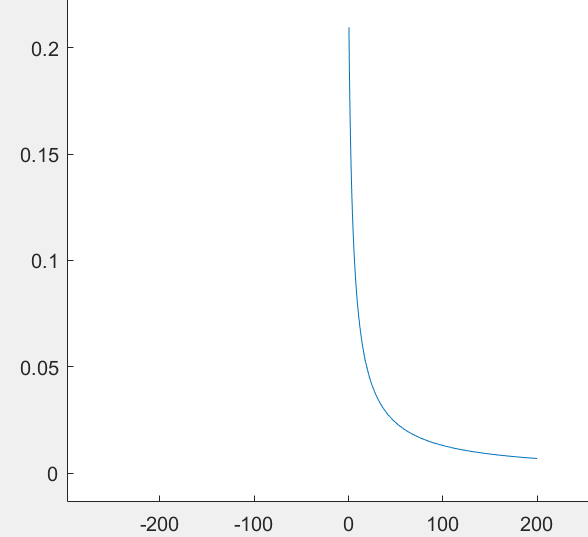
\includegraphics[width=8cm,height=5cm]{peak}
					\caption{感染比例的峰值随着$\gamma$的变化曲线}
				\end{figure}
	
	
	\section{SIR模型}
		\subsection{基本的SIR模型}
		
			\[\begin{cases}
			\frac{dS}{dt} = -\beta \frac{SI}{N} \\
			\frac{dI}{dt} = \beta \frac{SI}{N} - \gamma I \\
			\frac{dR}{dt} = \gamma I
			\end{cases}
			\]
			
			关于SIR三个量:由于SIR模型最终所有人都会感染病毒,在武汉后期隔离措施做得足够好的情况下,这种情况显然不会发生。因此,我们取$N$代表可能感染的人群的数量,剔除掉那些在家完全没有感染风险的人群。即我们将这个系统等价到一个更小的总人数为$N$的系统。$S$仍然为易感人群,或者说是目前在$N$个人中还没有感染的人数,初值为$N$。我们仍然用$I$代表目前感染的人数,$R$代表康复的人数。
			
			关于参数: $\gamma$ 为平均治疗时长的倒数,我们取为$1/25$,即一个人从感染到完全康复的周期为25天左右。$\beta$为接触感染的概率,我们用实际数据去做最小二乘逼近来估计。
			
		\subsection{对武汉数据的实证检验}
			
			注意到在感染的初期,我们近似有:\[\frac{dI}{dt}=(\lambda-\gamma)I \Longrightarrow I =I_0 e^{ (\beta -  \gamma)t}  \]
			
			查找到武汉初期的感染数据:
			\begin{table}[H]
				\begin{center}
					\begin{tabular}{*{9}{c|}c}
						日期(1月)&22&23&24&25&26&27&28&29&30\\ \hline
						确诊人数$I$ & 45&62&198&258&425&495&572&618&698
					\end{tabular}
				\end{center}
			\end{table}
			
			然后用确诊人数增加的比例的均值来作为初期增长率$e^{(\beta-\gamma)}$近似,即\[\frac18 \sum_{k=i}^8\frac{I(k+1)}{I(k)} \approx e^{\beta-\gamma}\]
			由此计算出初期的感染率大约为$\beta=0.4812$
			
			然后对于初始人数$N$,我们在区间[40000,1000000]间,以1000人为步长枚举,每次用Matlab中ode45包解微分方程,然后选择与原始56天的数据点数据平方偏差最小的值。最后我们得到的结果为$N=51000$。即总共有51000人感染。这与武汉的3月30日的数据(累计50006人确诊)还是很接近的。
			\begin{figure}[H]
				\begin{center}
					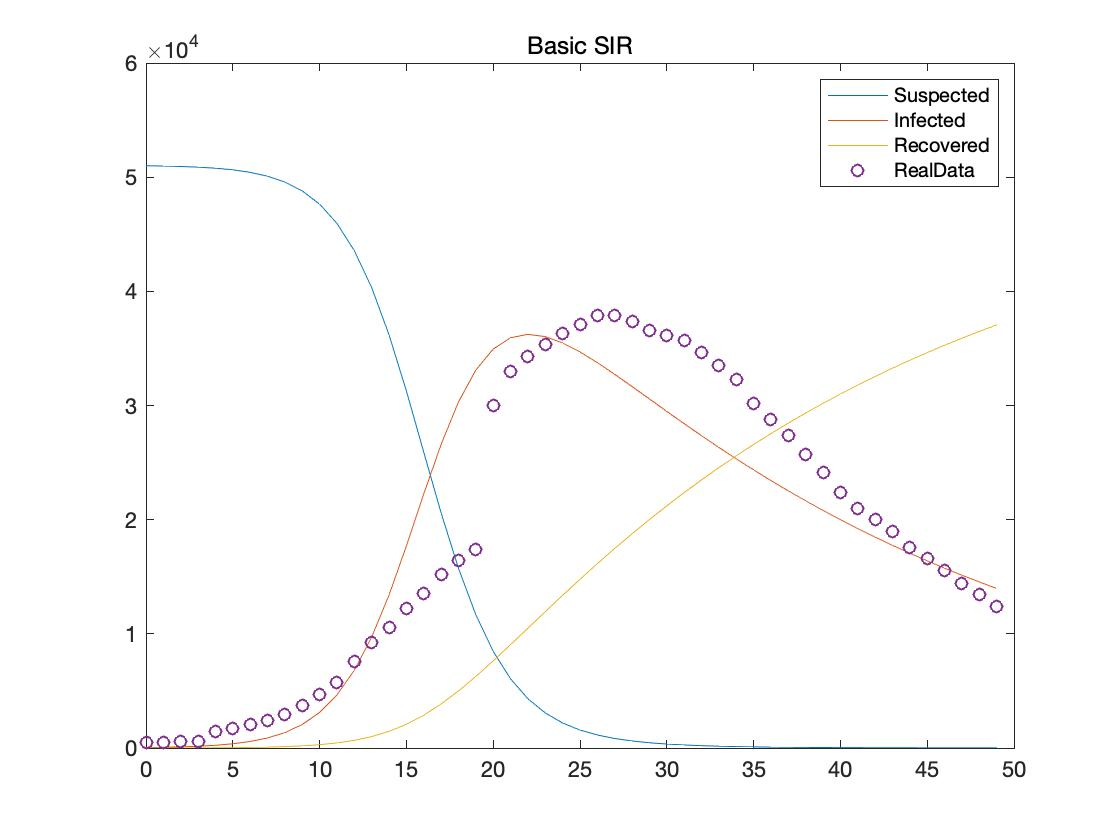
\includegraphics[scale=0.3]{Basic_SIR}
					\caption{基础SIR模型,$N=51000,\beta=0.48,\gamma=1/25$}
				\end{center}
			\end{figure}
		
		\subsection{SIR模型的数值敏感度}
			SIR模型中最重要的传染病变量为传播率$\beta$,而降低$\beta$的取值也是控制传染病的根本途径,我们在这一节中探究SIR模型对$\beta$的数值敏感度,以对武汉的隔离封城措施提供理论依据。
			
			我们仍然假设总人数$N=51000$,同样的,在SIR模型中,所有人最终都会被感染,因此,我们主要比较感染人数峰值的变化。峰值的大小也对传染病的防治至关重要,因为它意味着一个地区的医疗水平是否能够应对这次疫情的冲击。当峰值比较低且很缓时,这个传染病相对是比较容易应对的。反之的话医疗资源便会面临严重短缺,酿成重大灾难。
			
			我们分别取$\beta = 0.36,0.24, 0.12, 0.06$四个值,即分别将$\beta$缩小到原来的$\frac34, \frac 12 ,\frac14 ,\frac18$。得到的结果如图3。
			
			\begin{figure}[H]
				\centering
				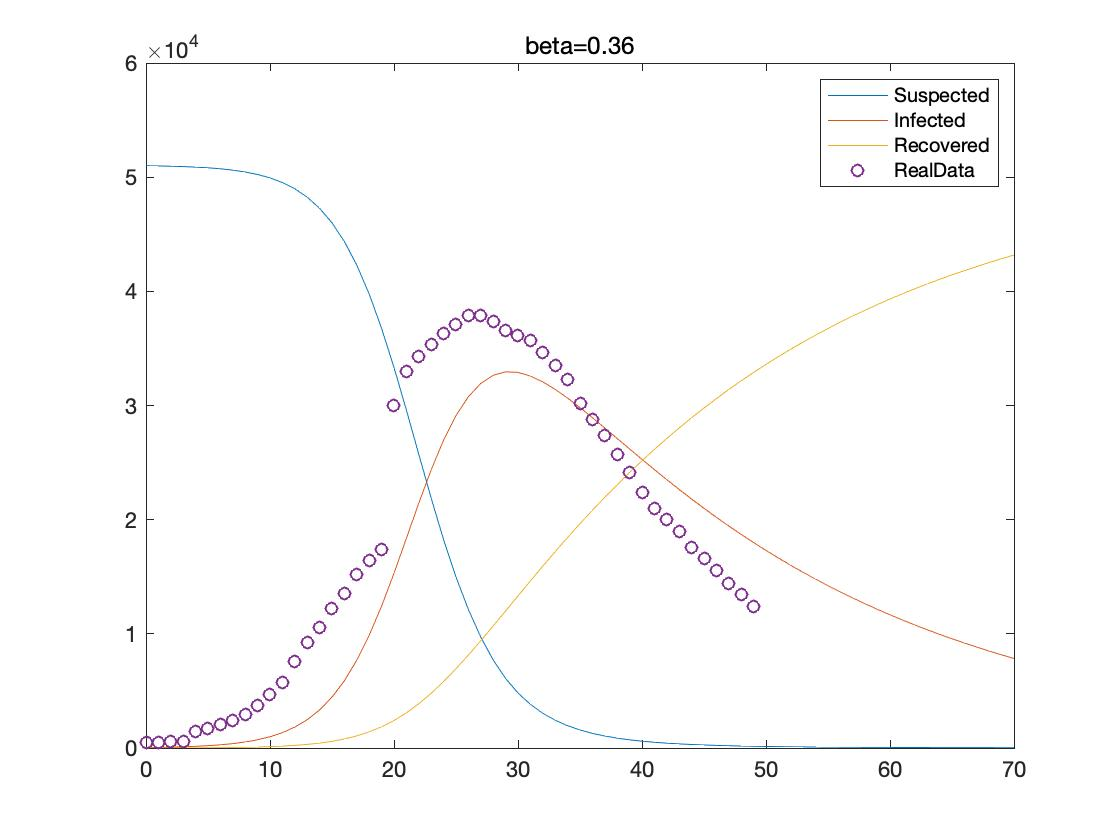
\includegraphics[scale=0.15]{beta4.jpg}
				\qquad
				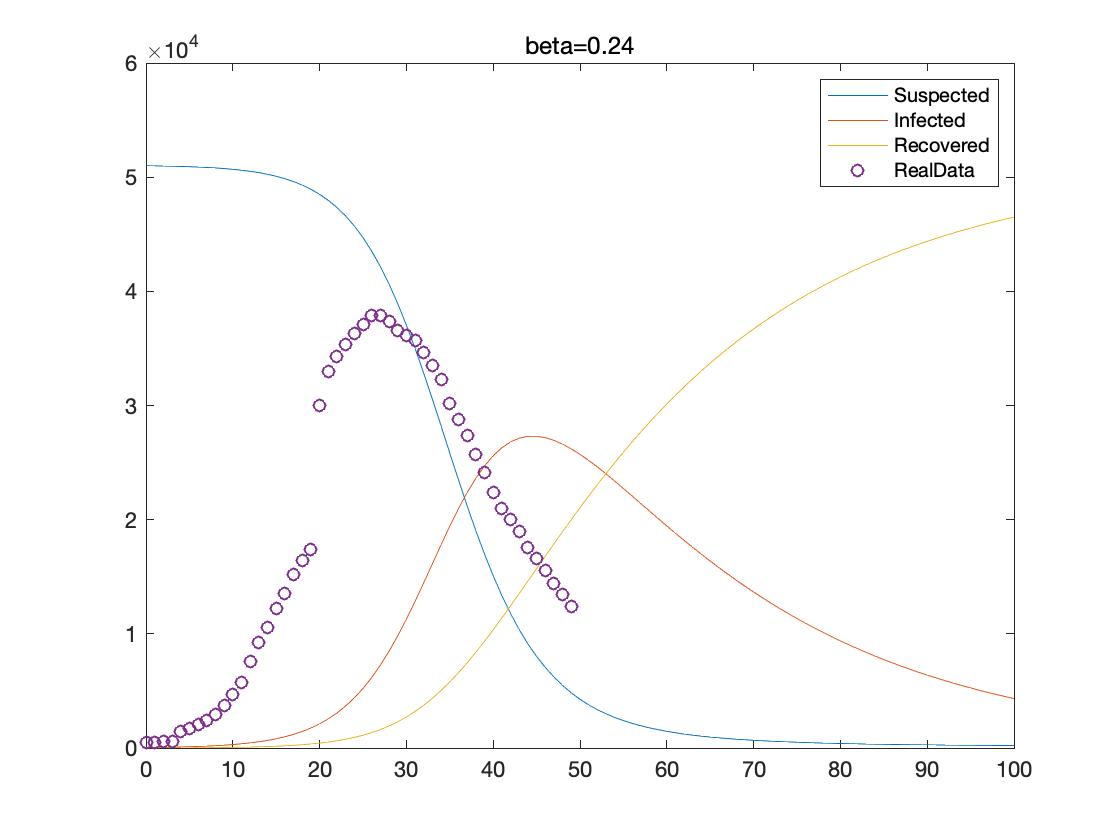
\includegraphics[scale=0.15]{beta3.jpg} \\
				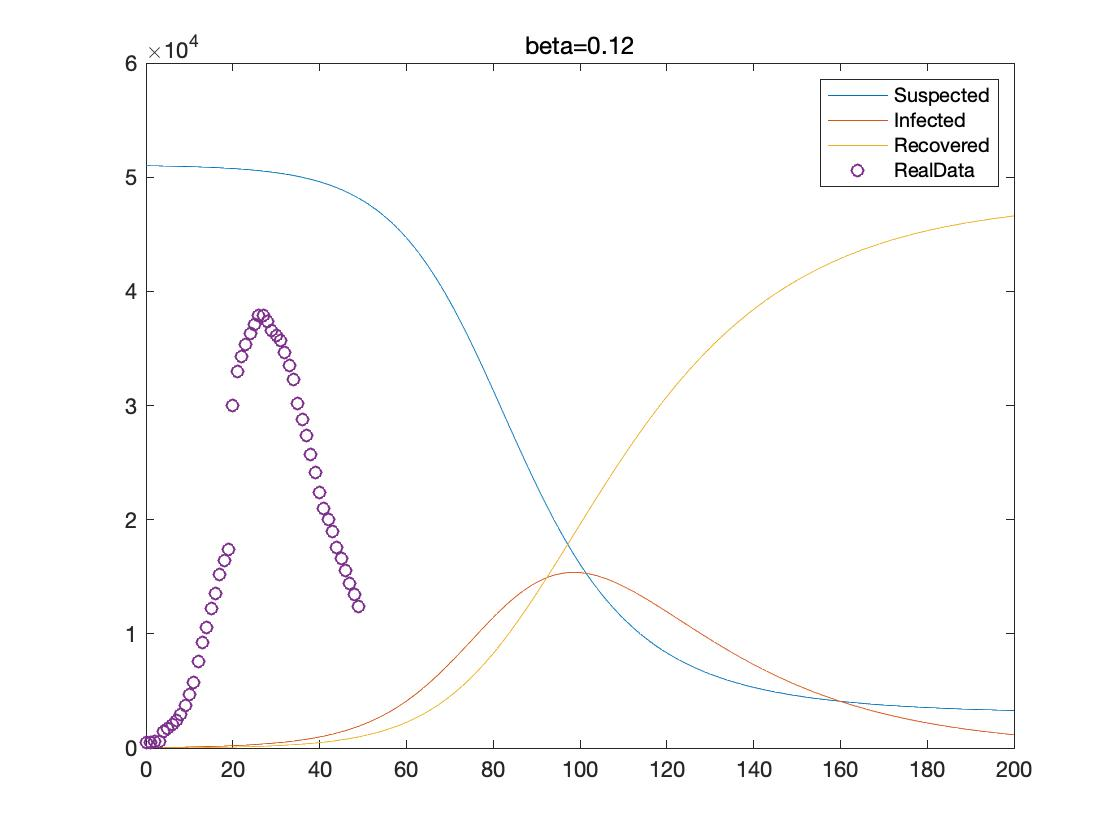
\includegraphics[scale=0.15]{beta2}
				\qquad
				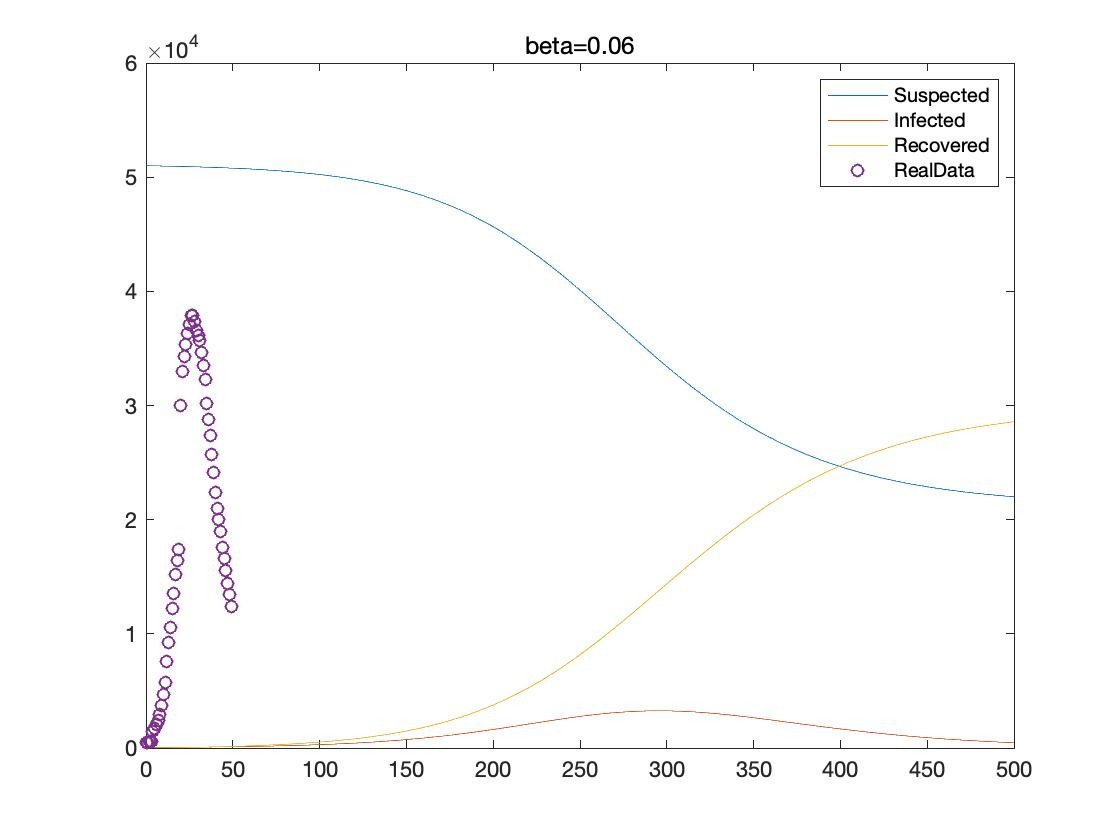
\includegraphics[scale=0.15]{beta1}
				\caption{不同$\beta$对峰值的影响对比}
			\end{figure}
			
			可以看到,当$\beta$值减小到一半时,峰值会减小大约$\frac13$。而当$\beta=0.12$时,峰值已经有了显著的降低。$\beta$更小时峰值更是可以忽略不计。相应的,达到峰值的时间我们也简单归纳如表1
			\begin{table}[H]
				\begin{center}
					\begin{tabular}{*{5}{c|}c}
						$\beta$&0.48&0.36&0.24&0.12&0.06 \\ \hline
						峰值时间&22&30&42&98&289
					\end{tabular}
				\end{center}
				\caption{$\beta$对峰值时间的影响}
			\end{table}
		
			可以看出,$\beta$的值对峰值到达时间的延迟的作用是显著的。而峰值到达时间的延迟意味着更多的准备时间,这便可以降低疫情的影响。而我们从图2中看出,实际的感染人数峰值到达时间在预期之后,可见武汉初期的封城措施还是起到了一定的效果。
		
		
	\section{SEIR模型}
		\subsection{模型}
			\[
			\begin{cases}
			{\frac{\mathrm{d}S}{\mathrm{d}t} = -k_1\frac{SI}{N}}\\
			{\frac{\mathrm{d}E}{\mathrm{d}t} = k_1\frac{SI}{N} - \epsilon E}\\
			{\frac{\mathrm{d}I}{\mathrm{d}t} = \epsilon E - \gamma I}\\
			{\frac{\mathrm{d}R}{\mathrm{d}t} = \gamma I}\\
			\end{cases}
			\]
		
		\subsubsection{模型解释}
			这是意义略不同的SEIR模型:
			
			S:易感人群
			
			E:已感染潜伏期
			
			I:发病有感染力
			
			R:发病无感染力(理想情况对应累计确诊,即一旦确诊就被收治,无法感染别人)
			
			注:这个模型不关心治愈和死亡
			
			
		\subsubsection{参数意义}
		$k_1$:在感染人数很少时平均一个有感染力的人一天能感染多少人
		
		$\epsilon$:平均潜伏时间的倒数
		(参考值:$0.2$)
		
		$\gamma$:检测成功率
		(参考值:(核酸检测)$0.3-0.5$,实际值应该更小)
		
		\subsection{参数数值和模型初值}
		
			\subsubsection{$\epsilon$、$\gamma$的值}
				考察参数的实际意义,由于新冠肺炎一般潜伏期3-7天,取$\epsilon = 0.2$. 二月十二日以前武汉采用的是核酸检测双阳性确诊的确诊方法,此后采用的是结合胸部影像,即使核酸检测未双阳也计入临床确诊的办法. 当时相关专家认为核酸检测准确率为0.3-0.4,结合当时武汉大量病人不能及时接受核酸检测,以及医疗资源紧张,很多病人即使确诊也难以入院,移除率$\gamma$应该更小. 综合考虑实际确诊数据,二月十二日之前取$\gamma = 0.15$. 二月十二日之后取$\gamma = 0.6$. 
			
			\subsubsection{$S$、$E$、$I$、$R$的初值}
				我们从一月二十三日武汉封城开始考察,$R$初值就是当日累计确诊病例495,$I$取300,$E$取2000. 基于与SIR模型中同样的理由,我们并不取$N$ 为总人口10000000左右,而是等效的取整个疫情过程中受影响的人口,(这种假设的实际依据是在封城后人口流动性很小,实际的易感人群非常有限,例如在整个疫情过程中可能一栋居民楼没有出现感染者,又与外界几乎没有人员接触,那么这栋居民楼里的人实际上可以等效为不在武汉. 而对真正参与到疾病传播过程中的人来说,主要的传播途径为家庭聚集和医院交叉传播等聚集型传播,因此可以认为整个过程中$k_1$变化不大. )现在可以看到整个疫情过程中(如没有再次爆发)武汉总确诊人数约为50000,因此取$S$初值即$N$的值为50000.
			
			\subsubsection{$k_1$的值}
				$k_1$的值的意义是一个有传染力的感染者在周围都是非感染者时平均一天的传播人数,需要我们通过实际数据确定. 注意二月十二日变化确诊方法当天武汉新增确诊13436例,而一线医务人员反应肺部影响参与临床诊断准确率很高,因此二月十二日当天的$I$值应不比13436多太多. 结合$I$和$R$在二月十二日的值及实际数据,取$k_1 = 0.83$.
			
		\subsection{数值实验}
			用python的scipy库中的odeint函数给出模型中微分方程组初值问题的数值解,并画图.
			\begin{figure}
				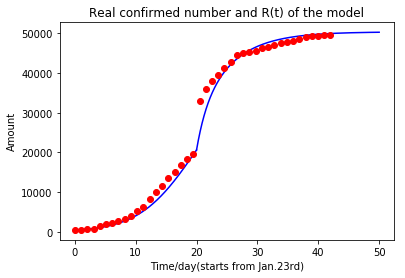
\includegraphics[scale=0.37]{real_and_R.png}
				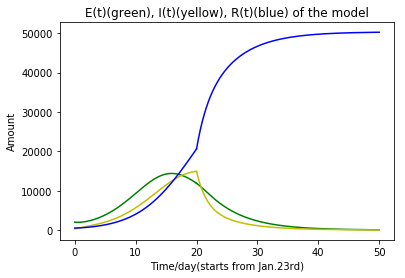
\includegraphics[scale=0.37]{EIR.png}
			\end{figure}
		
			可以看到模型确实能比较好地描述累计确诊人数的变化趋势,从模型给出的潜伏期人数$E(t)$和发病未收治人数$I(t)$的估计来看,第15天左右潜伏期人数达到峰值15000左右,而前二十天有感染能力的发病者人数一直上升,在第二十天(二月十二日)达到最大15000左右,此后立刻快速下降,这表现了改变确诊标准(实际作用时提高了发病者的移除率)的有益作用.
	
	\section{时滞模型}
		\subsection{模型的引入}
			\subsubsection{出现症状(未被确诊)的人群}
				影响疫情规模预测的一个重要因素为信息的延迟:
				传统SEIR模型以确诊人数作为感染人数进行参数反演,以确定$R_0$ 等参数。
				然而实际上,未确诊的患者并不一定处于潜伏期。
				由于医疗资源的缺乏,以及患者对于去医院会出现二次感染的顾虑,大部分患者经历的过程是:
				
				(\uppercase\expandafter{\romannumeral1}) 潜伏(未出现症状)$\Rightarrow$
				(\uppercase\expandafter{\romannumeral2}) 出现症状(未被确诊) $\Rightarrow$
				(\uppercase\expandafter{\romannumeral3}) 确诊
				
				出现症状以后,绝大部分患者会进行自我隔离,减少出行,传染性随之大幅降低。
				故\uppercase\expandafter{\romannumeral2}阶段与通常SEIR 模型中的潜伏期有很大不同,
				不能简单将\uppercase\expandafter{\romannumeral2} 阶段视作处于潜伏期。
				同时,二月十二日,将临床诊断纳入确诊数据后,一天内确诊人数增长了一万多例。
				由此可以看出,有大量的患者处于\uppercase\expandafter{\romannumeral2}阶段,即出现轻症但未被确诊。
				故处于这一阶段的人群不能被简单地忽视掉。所以用传统SEIR 模型进行参数反演与结果预测时,会出现较大的偏差。
				为此,我们参考The reproductive number R0 of COVID-19 based on estimate of a statistical
				time delay dynamical system. Nian Shao et al.一文中提出Fudan-CDCC的模型,并对Fudan-CDCC模型的不合理之处做了修正。
	
			\subsubsection{时滞的引入}
				在之前叙述的患者的三个过程里,我们不再假定
				(\uppercase\expandafter{\romannumeral1})$\Rightarrow$
				(\uppercase\expandafter{\romannumeral2})$\Rightarrow$
				(\uppercase\expandafter{\romannumeral3})
				是以恒定速率变化的,而是采用分布函数描述从上一过程进展到下一过程所需的时间:
				
				$T_2$:描述(\uppercase\expandafter{\romannumeral1})$\Rightarrow$(\uppercase\expandafter{\romannumeral2}) 所经历的时间
				
				$T_3$:描述(\uppercase\expandafter{\romannumeral2})$\Rightarrow$(\uppercase\expandafter{\romannumeral3}) 所经历的时间
				
				$T_4$:描述从出现症状到被隔离所需的时间。有$T_4=T_2+T_3$。
				
				设$T_2 \sim f_2$ $T_3 \sim f_3$ $T_4 \sim f_4$
				注意到 $f_4(t)=\int_0^t f_2(t-s)f_3(s)ds$
				
				现在的问题是确定$T_2$与$T_3$的分布,由于难以获得一手数据,我们通过
				Early Transmission Dynamics in Wuhan, China, of Novel Coronavirus–Infected Pneumonia Qun Li et al文章中根据早期十名患者的就诊信息推断出的结果:
				$$f_2(t)=\frac{1}{\sqrt{2\pi} \sigma t} exp{-\frac{log(t)-\lambda}{2 \sigma^2}} \ with\  \lambda=1.417\ \sigma^2=0.4525$$
				$$f_3(t)=(\frac{k}{\lambda})(\frac{t}{\lambda})^{k-1} e^{-(\frac{t}{\lambda})^k}\ with\ \lambda=10.836\ k=2.711$$
				这样,通过计算就可以得到$f_4$。
	
		\subsection{具体模型}
			传统SEIR模型中引入总人口与治愈死亡人数。
			然而在本次疫情中,感染人数远小于总人口,故我们将传统模型简化,仅考虑感染者人数,将上面所述的三个阶段作为三个变量。
			定义$I(t)$代表$t$时刻感染的总人数。$G(t)$代表$t$ 时刻未被确诊但已经被隔离的感染者。 $J(t)$代表$t$ 时刻确诊的感染者。
			$I_0=I-J-G$为感染者中未被隔离的人数,这一部分人具有感染性,设感染系数为$r$,
			则$rI_0(t)$可以代表$t$时刻新增的感染数。
			由此立马得到,$rI_0(t_1)f_2(t_2)$可以代表第$t_1$ 时刻被感染的人在$t_1+t_2$时刻就诊的人数
			固定$t_1+t_2$,对$t_1$从$0$积到$t_1+t_2$,便可以得到新增确诊人数。
			
			出现症状之后,患者本身及大量的密切接触者会进行居家隔离,而密切接触者中处于潜伏期感染者的比例很高。
			故平均每发现一个轻症患者,都会导致多个感染者被隔离。
			我们用$\beta(t)$表示隔离的感染者与出现症状的感染者之比,注意这是一个很可能大于1的比值。
			则与$J$同理,$\int_0^t rI_0(t-s)(f_2(s)-f_4(s)) ds$ 代表$t$时刻新增出现症状(去除掉了确诊的患者)的人数。
			乘上$\beta(t)$以后,就可以得到$G$的人数。
			具体模型为:
			$$\frac{dI}{dt}=r(I(t)-G(t)-J(t))$$
			$$\frac{dJ}{dt}=\int_0^t rI_0(t-s)f_4(s) ds $$
			$$\frac{dG}{dt}=\beta(t)\int_0^t rI_0(t-s)(f_2(s)-f_4(s)) ds $$
			其中$\frac{dG}{dt}$中加入了我们对Fudan-CDCC做出的修正。
	
		\subsection{求解模型}
				由于这个微分方程过于复杂,我们采用离散化的方法求解,得到的式子为
				$$I(t+1)=I(t)+r(I(t)-G(t)-J(t))$$
				$$J(t+1)=J(t)+\sum_{s=1}^{t-1} I_0(t-s)f_4(s) $$
				$$G(t+1)=G(t)+\beta(t) \sum_{s=1}^{t-1} rI_0(t-s)(f_2(s)-f_4(s)) $$
				
				取疫情开始节点为十二月十九号,当天的所有感染者$I(1)=7$。
				考虑到国家隔离政策的变化,取感染率和隔离参数如下:
				$$r=0.3122\ (t>33),\ r=0.272\ (t\leq33)$$
				$$\beta(t)=1.4\ (t>33),\ \beta=0\ (t\leq33)$$
				得到如下结果:
	
				\centerline{
\includegraphics[scale=0.3]{1.png}}
				
				
				图像中蓝线为实际感染人数$I$,红线为国家卫健委发布的确诊数据,可以看出,本模型较好地体现了时滞效应。
				
				本模型中的一个关键参量是$\beta$,如果只隔离轻症患者与确诊者,
				不隔离与他们密切接触的人群,即$\beta<1$,
				在病毒传播早期,$I_0(t)$单增,设$\frac{dI_0}{dt}(t_0)=0$,$t_0$是感染人数增长的拐点
				
				$$\frac{d(G+J)}{dt}(t_0)=\int_0^{t_0} \beta(t) rI_0(t_0-s)(f_2(s)-f_4(s))+rI_0(t_0-s)f_4(s) ds$$
				$$< \int_0^{t_0} rI_0(t_0-s)f_2(s)ds=\int_0^{t_0} \frac{dI}{dt}(t_0-s) f_2(s)ds$$
				$$< \int_0^{t_0} \frac{dI}{dt}(t_0) f_2(s) ds < \frac{dI}{dt}(t_0)$$
				
				倒数第二步是借助了$I_0(t)$当$t<t_0$的单增性。不等号都是严格小于,我们得到
				$$\frac{d(I-G-J)}{dt}(t_0)>0$$
				即$\frac{dI_0}{dt}(t_0)>0$,与假设$\frac{dI_0}{dt}(t_0)=0$矛盾,这说明恒有$\frac{d^2I}{dt^2}>0$
				甚至连疫情的拐点都无法到来。
				当然,这是由于我们的模型中没有考虑总人数,当$\beta$<1 的时候感染人数以指数级增长。
				$\beta=0.9$时结果如下图
				

					\centerline{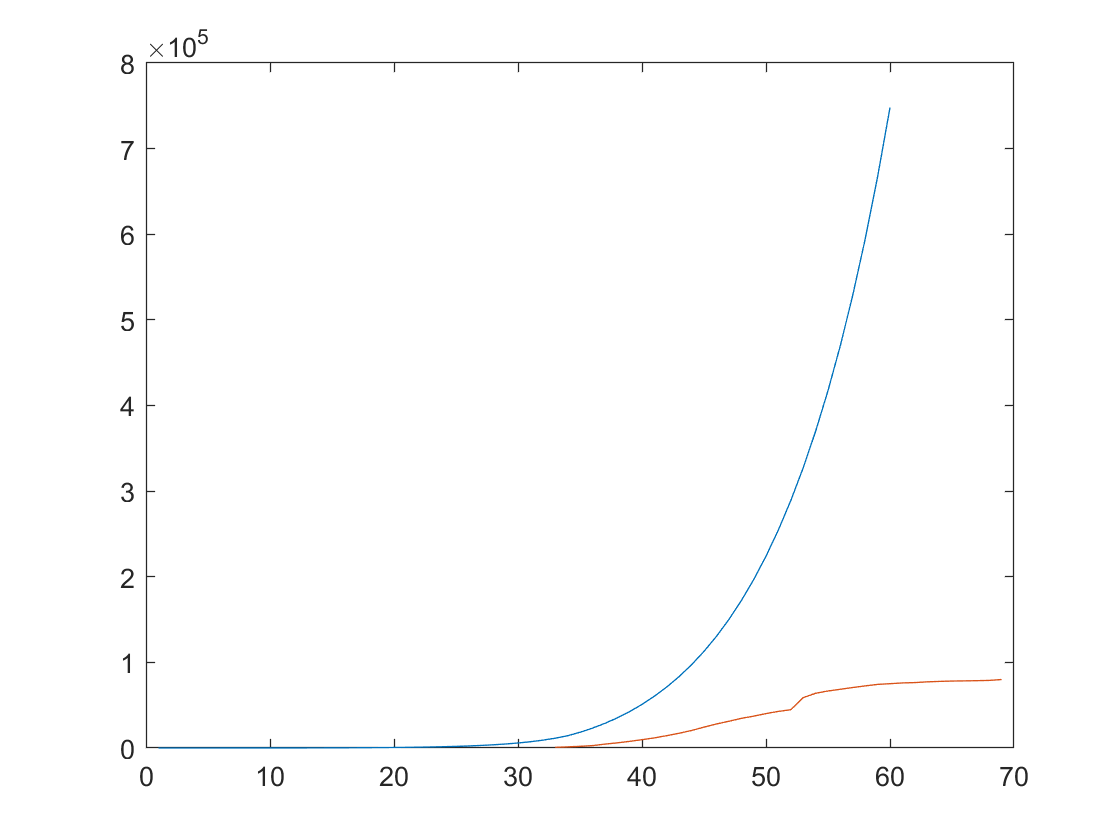
\includegraphics[scale=0.3]{2.png}}
					
				
				
				由此可见,仅仅隔离出现症状的感染者是无法控制疫情的。
	
		\subsection{对模型的进一步改进}
			\subsubsection{修改后的模型}
				在求解上述模型中,我们在拟合参数时遇到了巨大的困难,
				这促使我们怀疑Fudan-CDCC模型本身存在一定的问题,为此我们尝试做出进一步修正:
				
				\indent 在原模型中,$\beta$需要达到一个远大于1 的值才能使总感染人数不收敛到正无穷;但实际情况中迎来疫情拐点所需要的$\beta$却远小于理论值。事实上,这是因为该模型忽视了政府出台的限制出行等措施对无症状感染者隔离率的影响,而直接认为无症状感染者的隔离只取决于有症状感染者。当无症状感染者的比例足够大的时候,即使积极搜寻密切接触者使得$\beta$ 达到一个较高的值,无症状感染者的“隔离率”仍然会很小,这显然不符合现实。
				事实上这是因为各国政府在抗击新冠疫情的时候,不仅会试图隔离密切接触者,还会对民众的出行、聚集进行一定的限制。
				
				\indent 在修正的模型中,为了更好地模拟政府防疫措施的出台对人们接触机会减少的影响,我们引入隔离率$S(t)$,它代表人们相互接触的次数的减少比例。更加精确的表述是,$(1-S(t))r$代表了单位时间内一个无症状患者能够感染人的数量。随着政府出台越来越严格的封锁措施,$S(t)$将在一段时间内单增;由于政府出台政策是一个离散的过程,我们不妨认为$S(t)$ 是一个阶梯型的函数。同时,我们不妨认为所有感染者都会经历无症状- 轻症自我隔离- 确诊,即
				(\uppercase\expandafter{\romannumeral1})$\Rightarrow$
				(\uppercase\expandafter{\romannumeral2})$\Rightarrow$
				(\uppercase\expandafter{\romannumeral3})这个过程。为了方便表述和理解,我们记无症状感染者转轻症患者的速率为$N(t)$。
				
				\indent 为了更明显地看出政府的封锁措施的影响,我们可以暂时不考虑对密切接触者的排查。事实上,这种排查的影响在大多数情况下几乎等效于隔离率$S(t)$的增大,故我们只用考虑$S(t)$的影响,而不用考虑$\beta$ 对结果的影响。
				具体模型为:
				
				$$\frac{dI}{dt}=r(1-S(t))I_0(t)$$
				$$\frac{dJ}{dt}=\int_0^t N(t-s)f_3(s) ds $$
				$$\frac{dG}{dt}=N(t)-\int_0^t N(t-s)f_3(s) ds $$
				$$N(t)=\int_0^t r(1-S(t-s))I_0(t-s) f_2(s) ds$$
				
				由于这个微分方程过于复杂,我们采用离散化的方法求解,得到的式子为:
				$$I(t+1)=I(t)+r(1-S(t+1))I_0(t)$$
				$$J(t+1)=J(t)+\sum_{s=0}^{t+1} N(t+1-s)f_3(s) $$
				$$G(t+1)=G(t)+N(t)-\sum_{s=0}^{t+1}N(t+1-s)f_3(s)$$
				$$N(t+1)=\sum_{s=0}^{t+1}r(1-S(t+1-s))I_0(t-s)f_2(s)$$
				$$I_0(t)=I(t)-J(t)-G(t)$$
	
			\subsubsection{参数调试与结果}
				我们以美国为例。假定首批无症状感染者$I(0)=4$,首先我们由$S(t)$ 的定义知,任何国家在疫情发展的前期$S(t)$ 都是0,据此我们可以根据总确诊病例$J$在前期的增长得出$r$的近似值。我们先来看一下美国3 月1 日起的总确诊病例数:
			\begin{table}[H]
				\centering
				\caption{美国3月1日起的总确诊病例:}
				\begin{tabular}{|c|c|c|c|c|c|c|c|c|c|}
					\hline
					日期&4&5&6&7&8&9&10&11&12\\ \hline
					人数&160&236&335&447&572&728&1004&1322&1666\\
					\hline
				\end{tabular}
			\end{table}
			
			我们选取这一段的数据进行拟合,因为在3月之前美国的确诊病例主要来源于境外输入,且CDC的数据常常一连几天不更新,这会使我们难以得到正确的数据;而这一阶段的数据较好地体现了在$S(t)=0$ 时的病例增长情况。我们将感染系数$r$的值从0.375开始以0.005为步长枚举到0.475,得到的最小二乘估计是0.455。在这个感染系数下,$J(t)$的一部分数据如下:
			\begin{table}[H]
				\centering
				\caption{$r=0.455$下的病例增长:}
				\begin{tabular}{|c|c|c|c|c|c|c|c|c|c|}
					\hline
					日期&24&25&26&27&28&29&30&31&32\\ \hline
					人数&198&261&343&450&587&766&997&1296&1682\\
					\hline
				\end{tabular}
			\end{table}
			
			同时我们知道作为疫情“震中”的纽约市在3月13日要求酒吧餐厅容纳人数不能超过承载力的一半;3月20日美国实施了全面保持社交距离的措施,在加利福尼亚州命令将近4千万人待在家中后,美国纽约州、伊利诺伊州和康涅狄格州20 日也都宣布要求所有非必要到岗的工作人员待在家中。由于前者的强制程度较低,我们可以认为在3月13日左右$S(t)$有小幅增长,而3 月20 日$S (t)$受政策影响将会大幅增长。同时考虑到美国人民对政府的信任度,我们认为在政府出台最严格防疫措施之后一周人们才会自觉地待在家里。根据3月13日到4 月3 日的数据我们可以估计出$ S_1(t)=0.1,S_2(t)=0.41,S_3(t)=0.66$。以下是根据如上估计得到的结果:
			

				\centerline{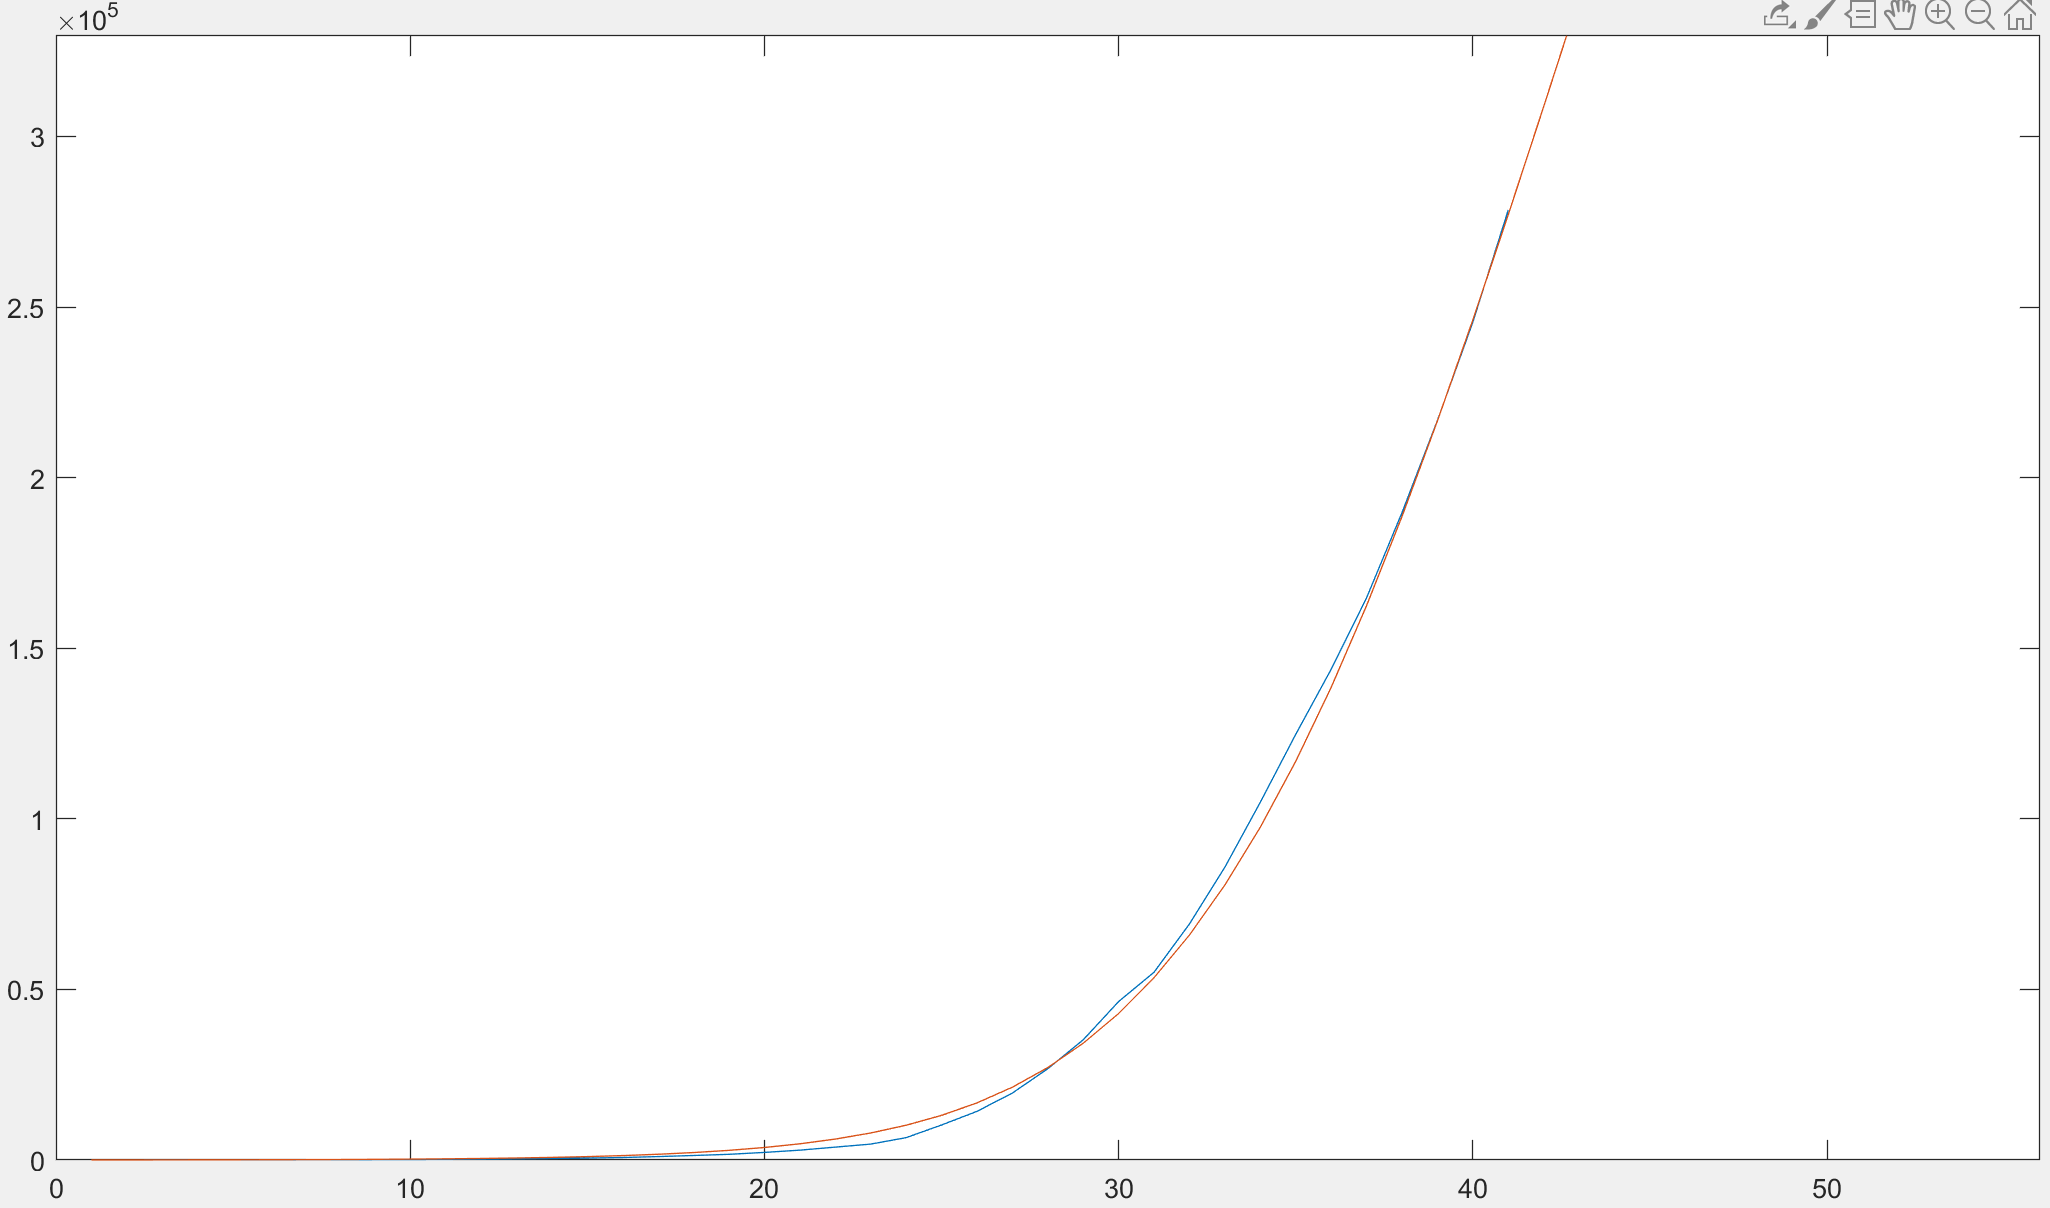
\includegraphics[scale=0.13]{3.png}}
				

			
			其中蓝线是实际确诊人数,而红线是此模型对实际数据的拟合。我们对两条曲线进行了沿$x$轴方向的平移使得它们的相似度更加明显。事实上我们可以从图中明显地看出时滞效应:隔离率$S$的增长发生在图中$x=17,24,31$的地方,但是确诊病例数在$x<39$时仍在加速增长,直到$x=39$时我们才能观察到新增确诊数趋于恒定。按照这个模型估计,美国的新增病例数将在$x=50$左右开始逐渐下降。
	
			\subsubsection{该模型的数值敏感度}
				按照我们刚才的估计,美国的确诊病例增长如下图所示:
				
				\begin{figure}[H]
					\centering
					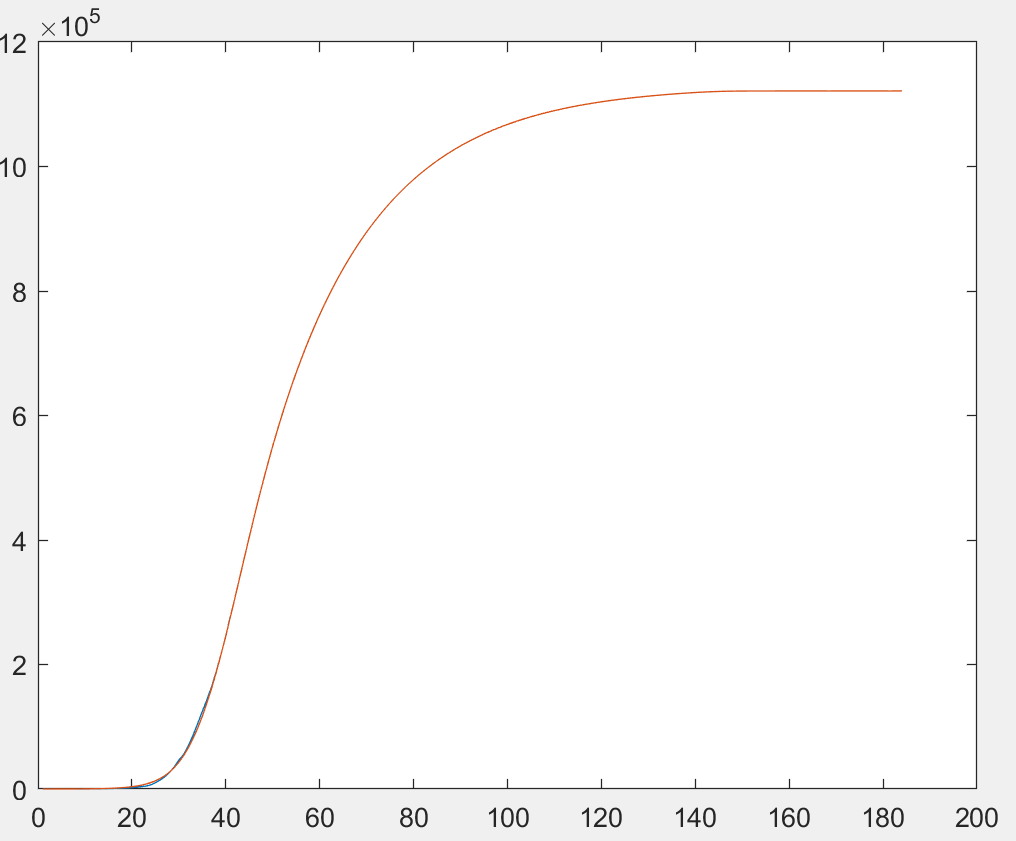
\includegraphics[scale=0.25]{4.png}
					
				\end{figure}
				
				最终美国的确诊病例数可能达到112万。如果我们假设民众对政府防疫措施的反应更加积极,比如只需要6天,人们就会自觉地待在家里,即阶梯函数$S(t)$ 的第三次增长距离第二次增长只有6天,那么我们可以画出如下的预测图像:
				
		
					\centerline{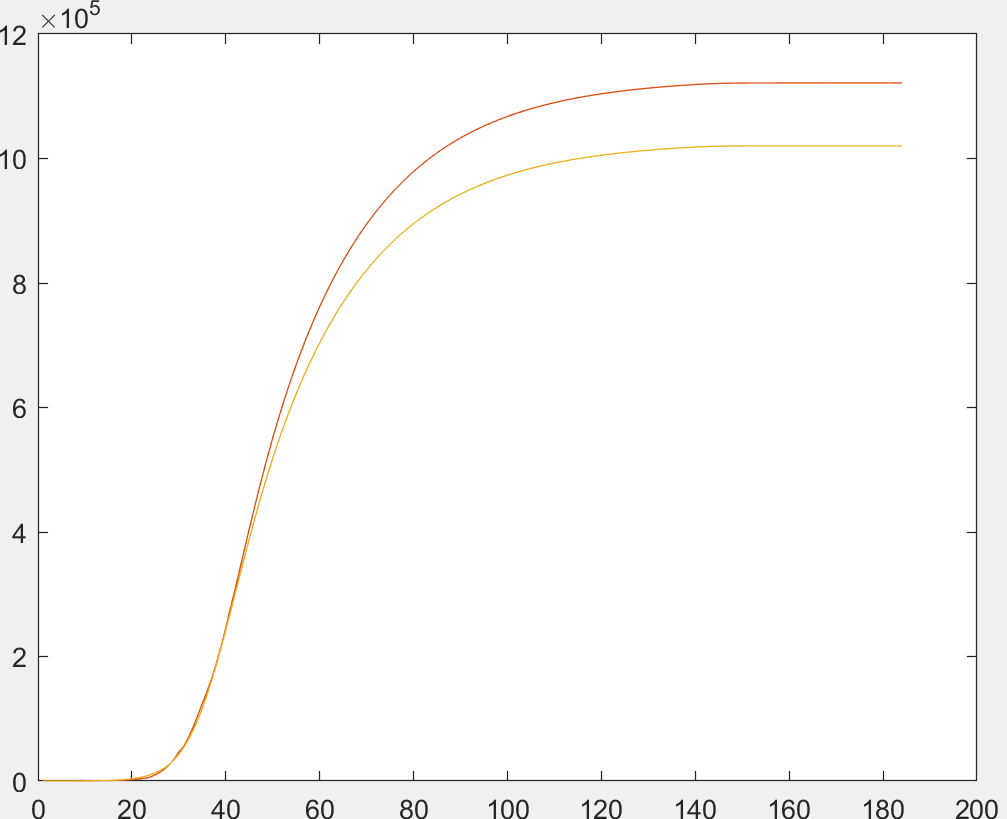
\includegraphics[scale=0.25]{5.png}}
		
				
				令人惊奇的是,最终的确诊人数直接降到了102万!即使民众早一天意识到新冠肺炎的严重性,都有可能拯救上万个人的生命。事实上其它参数的改变也会对结果产生极大的影响,以下我们通过列表的方式体现这种数值上的不稳定性:
				
				\indent 以下是感染系数对最终确诊人数的影响。从这张表中可以看出0.2\%的感染系数变化都可以导致4\%以上的总感染人数变化。
				
				\begin{table}[H]
					\centering
					\caption{}
					\begin{tabular}{|c|c|c|c|c|c|}
						\hline
						感染系数&0.45&0.454&0.455&0.456&0.46\\ \hline
						确诊总人数&914615&1076347&1121317&1168236&1377234\\
						\hline
					\end{tabular}
				\end{table}
				
				\indent 以下是最终隔离率对最终确诊人数的影响。由这张表可以看出人们遵守政府防疫规定的必要性;即使人与人之间的接触增加一点都会导致确诊总人数的飞涨。同时这也充分体现了硬核防疫措施的必要性。
				
				\begin{table}[H]
					\centering
					\caption{}
					\begin{tabular}{|c|c|c|c|c|c|}
						\hline
						最终隔离率&0.65&0.659&0.66&0.661&0.67\\ \hline
						确诊总人数&1232368&1131156&1121317&1111695&1033434\\
						\hline
					\end{tabular}
				\end{table}
	\section{基于随机过程的传染病建模}
	
		\subsection{基于随机过程的传染病建模}
			
			在传统的常微分方程的模型中,我们是将人数连续化的。然而,实际的情况中,人数只能是整数。并且感染的过程带有某种随机性,这种随机性可能是由于个体不同或是环境的随机性带来的。因此,尽管之前的常微分方程的模型已经能够很好的刻画近似传染病的发生过程,这里我们还是基于随机过程构建出新的模型以揭示传染病的某些特点。
			
			
			\paragraph{模型}
			
			我们基于SIR模型,想通过连续时间参数的马氏链(\textbf{C}ontinuous
			\textbf{T}ime \textbf{M}arkov
			\textbf{C}hain)来表示状态空间的变化。因此马氏性要求我们做出如下假设:
			
			假设1(马氏性):对于一个事件 \(E\) , 定义它的速率为 \( r_E(t)\)
			,也就是说, 这个事件在时间区间 \((t, t+dt)\) 内事件 \(E\) 发生的概率为
			\(r_E(t)dt\). 马氏性假设要求 \(r_E(t)\) 不随时间变化而变化.
			
			由于指数分布是唯一具有再生性的连续性随机变量,
			因此这个假设实际上就要求了每个事件发生的概率分布为一个指数分布.
			
			假设2(简单性): 假设系统的总人数 \(N\) 不变, 也没有出生和死亡的现象;
			同类型事件发生的概率相同且独立.
			
			考虑传统的SIR模型中的$S,I$.
			
			\begin{equation}
			\begin{aligned}
			\frac{dS}{dt} &= -\beta SI \\
			\frac{dI}{dt} &= \beta SI-\alpha I
			\end{aligned} 
			\end{equation}
			
			对于新的随机SIR模型, (1) 右边的 \(\beta SI\) 项我们解释为\(S \to I\)
			事件的速率为 \(\beta SI\) . \( \alpha I\) 项解释为 \(I \to R \)
			事件的速率为 \(\alpha I \) . 因此我们得到了一个连续时间参数马氏链
			\(X_t =(S_t,I_t)\). 其状态空间为 \((\mathbb{Z}^{+})^2\)
			且转移速率矩阵由下式刻画:
			\begin{equation}
			q_{(s,i)(s-1,i+1)}=\beta s i, \quad q_{(s,i)(s,i-1)}=\alpha i
			\end{equation}
			
			这样一来, 就将基本SIR翻译成了随机过程的版本, 下面我们来具体分析这个模型.
			\begin{table}[H]
				\centering
				\begin{tabular}{c|c|c|c}
					事件 & 转移方向 & 速率 & 对\(I\)的作用\\ \hline
					感染 & \(S \to I\) & \(\beta SI\) & +1\\
					恢复 & \(I \to S\) & \(\alpha I\) & -1
				\end{tabular}
				\caption{随机SIR模型的信息}
				\label{tab:my_label}
			\end{table}
		
		
		\subsection{模型分析}
			
			
			\subparagraph{灭绝概率}
			
			由于 \(S+I\) 是不增的, 因此 \(X_t\) 是一个有限状态空间的 CTMC. 我们考虑
			\(X_t\)的嵌入链 \(\tilde X_t\), 即由 \(X_t\)
			的每次转移构成的一个离散时间的马氏链. 由于状态 \((s,0)\) 为吸收态, 若
			\(\tilde X_t\) 不触及吸收状态, 其限制在其它状态中的马氏链是不可约的,
			因而是常返的. 于是 \(\tilde X_t \) 到达 \((1,0)\) 无穷多次.
			由于\(\lim\limits_{n \to \infty}p^n =0,\ \ \forall p \in(0,1)\) .
			因而必然到达\((0,0)\) 矛盾. 于是我们知道 \(\tilde  X_t\)
			必然(以1概率)会触碰到吸收态. 即 \(X_t\) 必然到达吸收态.
			
			这也就是说, 这样一个传染病模型中的传染病必然会消失.
			
			
			\subparagraph{大规模人口情况}
			
			另一个我们很关注的情况就是在 \(N\) 很大时, 传染病的表现. 我们考虑比率
			\(s_t^N =S_t /N\) 和 \(i_t^N = I_t/N\) . 再假设 \(\beta = \nu/N\), 其中
			\(\nu\) 与 \(N\) 独立. 考虑一列模型 \(X_t^N\) , 选择 \(s_0^N \to s_0\)
			和 \(i_0^N \to i_0\) . 可以证明在 \(N \to \infty\) 时, 在 \( L_1\)
			意义下, \((s_t^N, i_t^N)\) 收敛到 \((s_t, i_t)\) , 也就是微分方程
			
			\begin{equation}
			\begin{aligned}
			(d/dt)s_t &= -\nu s_ti_t \\
			(d/dt)i_t &= \nu s_t i_t - \alpha i_t
			\end{aligned}
			\end{equation}
			
			的解. 注意到(3)与(1)是吻合的.因此在大规模人口的情况,
			分析odeSIR模型就可以近似模拟随机SIR模型. 这也进一步说明了随机SIR模型
			\(X_t\) 的合理性.
			
			
			\subparagraph{特殊情况分析}
			
			这里我们分析一种特殊情况:
			\(S_0 = N-1, I_0 =1, \lambda =1/N, \alpha = 0\)
			.也就是在无法治疗,无法自愈, 不至于死亡的情况下有一人染病.
			
			此时,如果由 \(i\) 个人已经染病, 那么就有 \(N-i\) 个人仍属于健康状态.
			那么下一个人被感染的速率是 \(q_i= i(N-i)/N\), 所需时间为
			\(t_i \sim \mathcal{E}(q_i)\) .
			所有人都患病所需的时间为\(T = \sum\limits_{i=1}^{N-1}t_i\).
			
			
			\begin{equation*}
			\begin{aligned}
			\mathbb{E}[T] &= \sum\limits_{i=1}^{N-1}\mathbb{E}[t_i]=\sum\limits_{i=1}^{N-1}q_i^{-1} \\
			&= \sum\limits_{i=1}^{N-1} \frac {N}{i(N-i)} = \sum\limits_{i=1}^{N-1}(\frac{1}{i}+ \frac{1}{N-i})\\
			&= 2\sum\limits_{i=1}^{N-1}\frac{1}{i} \approx 2\log{N}
			\end{aligned}
			\end{equation*}
			
			所有人都染病的期望时间为 \(O(\log{N})\) , 染病人数也就是成指数倍的增长.
			这种特殊情况让我们清楚的意识到如果疾病不能被及时治愈,
			那么带来的后果将会是灾难性的.
			
			
			\subparagraph{进一步简化}
			
			我们考虑两种事件\(S \to I\)和\(I \to R\)对\(I\)造成的影响,前者是\(I\)的值增加1,后者使\(I\)的值增加1. 因此,若只考虑\(I\)的值,可以得到一个类似于生灭链的过程.但是为了与随机过程中的生灭过程完全一致,我们需要如下假设.
			
			假设3(生灭过程):假设新增染病人数只与\(I\)的值有关,且\(S \to I\)事件速率与\(I\)成线性关系.
			
			那么我们就得到了一个生灭过程\(Y_t\):
			\begin{equation}
			q_{i,i+1}=bi,i \ge 0 \quad and \quad
			q_{i,i-1} = di, i >0
			\end{equation}
			这里的\(b\)可以视为每个患病者以独立地以速率\(b\)感染他人,\(d\)可以视为每个患病者独立地以速率\(d\)恢复. 那么许多有关于生灭链的结论都可以在此得到应用. 这里我们尤其关心何时\(Y_t\)会变为\(0\),也就是传染病彻底消失. 定义\(h(t) = \mathbb{P}(Y_t=0|Y_0 =1)\), 可以证明在\(b \neq d\) 时\(h(t)\)满足微分方程
			\begin{equation*}
			h(t) = \int_0^t \exp(-(b +d )s)\{d +b h(t-s)^2\}ds
			\end{equation*}
			进而求出\(h(t) = \frac{d e^{d t}-d e^{b t}}{d e^{d t}- b e^{b t}}\). 那么由生灭链的性质, \(\mathbb{P}(Y_t=0|Y_0 = n)= (h(t))^n\).固定\(d=1\)后,\(h(t)\)对不同\(b\)的函数图像如下.
			
			\begin{figure}[H]
				\centering
				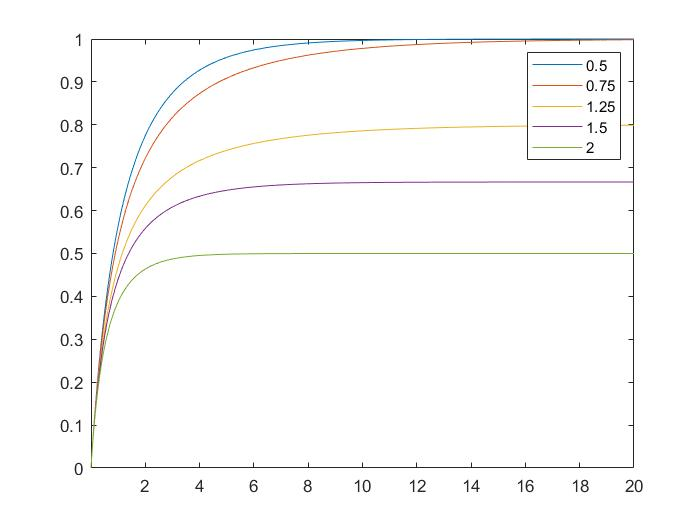
\includegraphics[width=0.5\linewidth]{pic.jpg}
				\caption{ \(\mathbb{P}(Y_t=0|Y_0 =1)\)在\(d=1\),不同\(b\)下的函数图像.}
				\label{fig:my_label}
			\end{figure}
			
			事实上,只要\(b <d\),则\(\lim_{t\to \infty}h(t) = 1\),即最终\(Y_t\)必然会变为\(0\), 但是\(b>d\)的时候,\(\lim_{t\to \infty} = d/b\),此时即有\(Y_t\)以正概率始终不为\(0\). 注意由于假设不同, 这里与上面之前讨论过的必然灭绝并没有矛盾. 这里的讨论再一次说明了传染性越强的疾病带来的破坏性越大.
		
		\subsection{总结}
			随机过程为我们看待疫情的传染带来了新的角度. 不像常微分方程那样会有一个解的存在, 随机过程刻画的是具有不确定性的动态的过程. 但是随机过程中总有许多整体的结构性的结论引人深思. 这方面还有许多更深刻的结论有待我们学习发现. 
			这一节已有的结论已经可以警醒我们.尽管有随机性, 疾病总会有概率消失, 但传染病的传播很有可能是十分猛烈的.生命只有一次,我们不能冒险, 唯有做好准备, 重视疫情,人类才有可能共同战胜一次又一次的传染病.
	\section{传染病模型中的最优控制问题}
		\subsection{最优控制问题简介}
			\indent 动态系统中的最优控制问题用于寻求一个控制函数使得目标泛函达到极值,特别地,对于一个常微分方程确定的系统,令$u(t)$表示控制函数,$x(t)$表示状态函数,控制函数对状态函数的影响可以表示为:
			\begin{equation}
			\begin{aligned}
			x'(t)=g(t,x(t),u(t))
			\end{aligned}
			\end{equation}
			\indent 我们的目标是寻求以下优化问题的解:
			\begin{equation}
			\begin{aligned}
			\max_{u\in L^1} \int_{0}^{T}f(t,x(t),u(t))dt
			\end{aligned}
			\end{equation}
			\indent 约束条件为:
			\begin{equation}
			\begin{aligned}
			x'(t)=g(t,x(t),u(t)),\ x(0)=x_0
			\end{aligned}
			\end{equation}
			\indent 对于这一类问题的求解,可以用类似于求函数最值中的Lagrange乘子法的方法求解,我们不加证明地给出以下结果,详细的讨论与证明请参考\cite{ref1}:
			\begin{theo}[Pontryagin's Maximum Principle]
				对于上述优化问题,设$u^*(t)$,\\ $x^*(t)$为优化问题的解,则存在伴随变量$\lambda(t)$,使得对于任意的$u\in L^1$,下式对于任意的时间$t\in[0,T]$成立:
				\begin{equation}
				\begin{aligned}
				H(t,x^*(t),u,\lambda(t))\leq H(t,x^*(t),u^*(t),\lambda(t))
				\end{aligned}
				\end{equation}
				其中Hamilton函数 H定义如下:
				\begin{equation}
				\begin{aligned}
				H(t,x(t),u(t),\lambda(t))=g(t,x(t),u(t))+\lambda(t)g(t,x(t),u(t))
				\end{aligned}
				\end{equation}
				且有:
				\begin{equation}
				\begin{aligned}
				&\lambda'(t)=-\frac{\partial H(t,x(t),u(t),\lambda(t))}{\partial x}\\
				&\lambda(T)=0
				\end{aligned}
				\end{equation}
			\end{theo}
		
		
		
		\indent 根据以上的定理,我们将原始的约束优化问题转化为了无约束优化问题,只需求$u^*(x)$使得$H$达到最大值,从而我们可以得到下面的推论,这一推论可以帮助我们实际求解优化问题。
		\begin{deduction}
			H在$u=u^*$处达到最大值的必要条件是:
			\begin{equation}
			\begin{aligned}
			&\frac{\partial H}{\partial u}=0\Rightarrow f_u+\lambda g_u =0&(optimal \ \ equation)\\
			&\lambda'=-\frac{\partial H}{\partial x}\Rightarrow \lambda'=-(f_x+\lambda g_x)&(adjoint \ \  equation)\\
			&\lambda(T)=0&(transversality \ \  condition)\\
			&\frac{\partial^2 H}{\partial u^2}\big|_{u=u^*}\leq 0&(second \ \ order \ \ condition)
			\end{aligned}
			\end{equation}	
		\end{deduction}
		
		\indent 对于方程组情形,我们也可以做类似的讨论,假设$\vec{x}(t)$是一个$n$维状态向量$\vec{u}(t)$是一个$m$维控制向量,我们的优化问题是:
		\begin{equation}
		\begin{aligned}
		&\max_{\vec{u}}\int_{t_0}^{t_1}f(t,\vec{x}(t),\vec{u}(t))dt+\phi(\vec{x}(t_1))\\
		&subject \ to \ \ \vec{x}\ '(t)=\vec{g}(t,\vec{x}(t),\vec{u}(t)),\vec{x}(t_0)=\vec{x}_0
		\end{aligned}
		\end{equation}
		\indent 设Hamilton函数$H(x)$为:
		\begin{equation}
		\begin{aligned}
		H(t,\vec{x},\vec{u},\vec{\lambda})=f(t,\vec{x},\vec{u})+\vec{\lambda}(t)\cdot \vec{g}(t,\vec{x},\vec{u})
		\end{aligned}
		\end{equation}
		\indent 同样可以得到一组必要条件:
		\begin{deduction}
			H在$\vec{u}=\vec{u}^*$处达到最大值的必要条件是:
			\begin{equation}
			\begin{aligned}
			&x_i'(t)=g_i(t,\vec{x},\vec{u}), \ x_i(t_0)=x_{i0} \ for \ i=1,2,\cdots,n\\
			&\lambda_j'(t)=-\frac{\partial H}{\partial x_j},\ \lambda_j(t_1)=\phi_{x_j}(\vec{x}(t_1)) \ for \ j=1,2,\cdots,n\\
			&\frac{\partial H}{\partial u_k} \ at \ u_k^*  \ for \ k=1,2,\cdots,m
			\end{aligned}
			\end{equation}	
		\end{deduction}
	
	
		\subsection{SIR模型中的疫苗分配优化问题}
	
		\indent 接下来我们应用上一节中的结果来解决具体的传染病模型中的优化问题,本节中我们具体考虑疫苗的分配问题,这里我们使用SIR模型:
		\begin{equation}\label{basis}
		\begin{split}
		S'(t)&=-\beta \frac{S(t)I(t)}{N}\\
		I'(t)&=\beta \frac{S(t)I(t)}{N}-\gamma I(t)\\
		R'(t)&=\gamma I(t)			
		\end{split}
		\end{equation}
		\indent 疫苗分配问题是指现在有一批疫苗,给易感人群$S$接种之后就可以将直接变成免疫人群$R$,在时间$T$内总共可以使用的疫苗数量为$X$,控制函数是易感人群$S$的接种率$u(t)$,目标函数为T时间内感染人数和接种疫苗的花费的和,具体的问题可以由下式给出:
		\begin{equation}
		\begin{split}
		\min_{u}&\int_{0}^{T}AI(t)+u^2(t)dt\\
		subject \ to \ :&\int_{0}^{T}S(t)u(t)dt=X\\
		&S'(t)=-\beta \frac{S(t)I(t)}{N}-u(t)S(t)\\
		&I'(t)=\beta \frac{S(t)I(t)}{N}-\gamma I(t)\\
		&R'(t)=\gamma I(t)+u(t)S(t)			
		\end{split}
		\end{equation}
		\indent 为了方便处理,我们可以定义函数$W(t)$将上面的积分约束转化为以下形式:
		\begin{equation}
		\begin{aligned}
		&W'(t)=S(t)u(t)\\
		&W(0)=0\\
		&W(T)=X
		\end{aligned}
		\end{equation}
		\indent 由于接种率有一定的限制,我们不妨假设接种率在[0,0.9]区间内,从而控制函数的集合为:
		\begin{equation}
		\begin{aligned}
		U=\{u:[0,T]\rightarrow[0,0.9]\ |\ u\ is \ Lebesgue \ measurable\}
		\end{aligned}
		\end{equation}
		\indent 接下来我们就可以使用前面介绍的Pontryagin's Maximum Principle来对这一问题求解,由于$R=N-S-I$恒成立,我们在考虑优化问题时可以忽略$R$的约束条件,我们首先定义Hamilton函数为:
		\begin{equation}
		\begin{aligned}
		H=AI+u^2+\lambda_{S}(-\beta \frac{SI}{N}-uS)+\lambda_{I}(\beta \frac{SI}{N}-\gamma I)+\lambda_{W}(Su)
		\end{aligned}
		\end{equation}
		\indent 使用ajoint equation可以得到:
		\begin{equation}
		\begin{aligned}
		&\lambda_{S}'=\lambda_{S}(\beta \frac{I}{N}+u)-\lambda_{I}\beta \frac{I}{N}-\lambda_{W}u,\  \  \lambda_{S}(T)=0 \\
		&\lambda_{I}'=-A+\lambda_{S}(\beta \frac{S}{N})-\lambda_{I}(\beta \frac{S}{N}-\gamma),\  \  \lambda_{I}(T)=0 \\
		&\lambda_{W}'=0
		\end{aligned}
		\end{equation}
		\indent 使用optimal equation可以得到:
		\begin{equation}
		\begin{aligned}
		&\frac{\partial H}{\partial u}\bigg|_{u^*}=0\\
		&\Rightarrow u^*(t)=\frac{S(t)(\lambda_{S}(t)-\lambda_{W}(t))}{2}
		\end{aligned}
		\end{equation}
		\indent 考虑函数族$U$的限制,可以得到:
		\begin{equation}
		\begin{aligned}
		u^*(t)=min\{0.9,max[0,\frac{S(t)(\lambda_{S}(t)-\lambda_{W}(t))}{2}]\}
		\end{aligned}
		\end{equation}
		\indent 解出最优控制函数后,我们的问题就转化为了求解方程组:
		\begin{equation}
		\begin{aligned}
		&S'(t)=-\beta \frac{S(t)I(t)}{N}-u(t)S(t), \ \ S(0)=S_{0}\\
		&I'(t)=\beta \frac{S(t)I(t)}{N}-\gamma I(t),\ \ I(0)=I_{0}\\
		&R'(t)=\gamma I(t)+u(t)S(t),\ \ R(0)=R_{0}\\
		&\lambda_{S}'(t)=\lambda_{S}(t)(\beta \frac{I(t)}{N(t)}+u(t))-\lambda_{I}(t)\beta \frac{I(t)}{N}-\lambda_{W}(t)u(t),\  \  \lambda_{S}(T)=0 \\
		&\lambda_{I}'(t)=-A+\lambda_{S}(t)(\beta \frac{S(t)}{N})-\lambda_{I}(t)(\beta \frac{S(t)}{N}-\gamma),\  \  \lambda_{I}(T)=0 \\
		&\lambda_{W}'(t)=0,\int_{0}^{T}S(t)u(t)=X\\
		&u(t)=min\{0.9,max[0,\frac{S(t)(\lambda_{S}(t)-\lambda_{W}(t))}{2}]\}
		\end{aligned}	
		\end{equation}
		\indent 方程组中共有六个方程,六个约束条件,可以利用一些数值方法解出最优控制函数下的解。
	\section{传染病建模的平均场网络模型}
	\subsection{概念模型建立}
	前面我们讨论了经典的SIR模型以及SEIR模型,以及利用时滞进行建模,但是这样的建模都缺少一个现实生活中必要的维度--空间;建模传染病地理传播最直接的方法是在SIR和SEIR模型基础上增加空间扩散,得出类似于理论生物化学反应-扩散方程的方程。该方法利用反应-扩散理论的工具对理解空间流行行为的一些基本方面是有用的,但存在明显的缺陷,比如人类的行为远比一个粒子运动要复杂,这是一个主要的复杂性,导致了复杂的积分-微分方程,其中扩散部分与反应部分相互作用,即传递。
	\par 为了解决上述问题,我们将大量人口分割成有限数量的区块,每个区块遵循自己的确定性“局部”流行病模型;地方动态通过人口流动联系在一起。通过不同区块之间的相互联系,有利于传染病的地理传播和持续传播。我们考虑以下系统,该系统具有$m$种流行病学状态(对于SEIR系统,$m=4$),在$n$个相互作用的区块中传播。如果区块是孤立的,则局部扩展由形式为$\dfrac{du_{j}}{dt}=f(u_{j})$的$n-m$维系统建模。在区块间存在线性人口流动时,一个区块具有以下相互关联的动力系统:
	\begin{equation}
		\begin{aligned}
			\dfrac{du_{j}}{dt}=f(u_{j})+\sum\limits_{i=1}^{n}c_{ij}Mu_{j}
		\end{aligned}
	\end{equation}
\par 其中$u_{j}$为与第$j$个区块有关的参量,$U=(u_{1},u_{2},\cdots ,u_{n})$为一个$m\times n$的矩阵;$M$为一个$m\times m$的对角矩阵,用于表示不同流行病学个体的不同迁移系数;$C$为一个$n\times n$的矩阵,代表着不同区块的个体之间的传输速率。
\par 我们考虑将SEIR模型改变,得到方程:
\begin{equation}
	\begin{aligned}
		&\dfrac{dS_{i}}{dt}=\mu (1-S_{i})-S_{i}\sum\limits_{j=1}^{n}\beta_{ij}I_{j}\\
		&\dfrac{dE_{i}}{dt}=S_{i}\sum\limits_{j=1}^{n}\beta_{ij}I_{j}-(\mu+\alpha)E_{i}\\
		&\dfrac{dI_{i}}{dt}=(\alpha-\mu-\gamma)I_{i}\\
		&R_{i}=1-S_{i}-I_{i}-E_{i}
	\end{aligned}
\end{equation}
\par 该描述的核心在于空间传播矩阵$\beta_{ij}$,它表示了一个i区块的易感者被区块j的感染者感染的人均比率。我们可以通过直接将区块的解释扩展到不同类型的内部同质群体,如社会群体、年龄群体等,仍然依赖于适当的接触或空间传播矩阵,比如具有反映社会群体或年龄群体之间不同接触模式的元素$\beta_{ij}$。
\subsection{传染病建模的网络模型}
现实的社会是异质个体的混合,这种异质性存在于几个方面,尤其是接触。我们之前的SIER模型的基础是基于全人群的随机混合,然而在实践中,每个人都有一组有限的接触者或他们可以传播感染的人,我们认为所有这些联系的集合形成了一个网络。这种个体间接触网络的结构模式允许模型从个体层面传播感染的过程计算人口规模的流行病动态。
\subsubsection{一些参数解释}
无向网络中顶点i的度$k_{i}$是由i发出的边数,在有向网络的情况下,我们用$k_{in}$和$k_{out}$分别作为结束于i或从i开始的边的数量。而有向网络的总度则由$k_{i}=k_{in}+k_{out}$定义。网络的度分布$P(k)$的概率是一个随机选择的顶点k的度,同理我们有$P^{in}(k_{in})$和$P^{out}(k_{out})$。
\par 两个顶点之间的度相关性定义为一条从k度顶点出发的边连接到$k_{0}$度顶点的条件概率$P(k_{0}|k)$。网络被称为不相关的如果这个条件概率是独立于原始顶点k。度相关最常用的度量方法是Pearson \quad correlation\quad coefficient\quad r,度相关系数定义为\footnote{M. E. J. Newman, Mixing patterns in networks, Phys. Rev. E 67 (2003) 026126.}:
\begin{equation}
	\begin{aligned}
		r=\sum\limits_{jk}\dfrac{jk(e_{jk}-q_{j}q_{k})}{\sigma^{2}},\quad \sigma^{2}=\sum\limits_{k}k^{2}q_{k}-[\sum\limits_{k}kq_{k}]^{2}
	\end{aligned}
\end{equation}
\par 其中$e_{ij}$为度相关矩阵,表示在随机选择的两端找到具有i和j度节点的概率,$q_{k}$为在随机选择的末端存在k度节点的概率。
\par \textbf{节点介数}:$b_{i}=\sum\limits_{j\neq k}\dfrac{n_{jk}(i)}{n_{jk}}$,其中$n_{jk}$是连接j到k的最短路径数,$n_{jk}(i)$是连接j到k并经过i的最短路径数。
\par \textbf{平均值}:对于网络中的元素,我们定义其平均值为$\left\langle c\right\rangle=\sum\limits_{k}P(k)c(k)$
\par \textbf{无标度网络(SF)}:现实世界的网络是由一个节点层次结构构成的,只有少数节点具有非常大的连接性,而绝大多数节点的度要小得多,通常近似于形式为$P(k)\sim k^{-\zeta}$的幂律行为\footnote{M. E. Newman, Properties of highly clustered networks, Physical Review E 68 (2) (2003) 026121.},这意味着找到具有非常大的度的顶点的概率不可忽略。
\subsubsection{传染病网络模型的初步建立}
传统的流行病模型,如经典的SIS或SIR流行病模型假设任何个体都可以与任何其他个体接触,因此所有个体的接触次数都是相当的。它还假设网络中所有个体的疾病传播概率是相同的。这两种假设在大多数疾病中都是有限的:在现实中,一个人只能将病原体传播给他接触过的人,而且传播的概率也各不相同。因此,可以假定病原体在复杂的接触网络中传播。
\par 我们首先考虑一个具有均匀恢复速率$\gamma$的SIR模型,即感染节点在感染后以速率$\gamma$被切除,感染速率$\beta_{I}$。那么传染性T被定义为在恢复之前,感染将从一个被感染节点传播到一个连接的易感邻居的概率;则传递率计算为:
\begin{equation}
	\begin{aligned}
		T=1-\lim\limits_{\delta t\to 0}(1-\beta_{I}\delta t)^{\gamma/\delta t}=1-e^{-\gamma\beta_{I}}
	\end{aligned}
\end{equation}
\par 而其实实际上的$\beta_{I}$和$\gamma$对于不同个体而言是不同的,因此我们应该取传递率的平均值为\footnote{M. E. Newman, Spread of epidemic disease on networks, Physical Review E 66 (1) (2002) 016128.}:
\begin{equation}
	\begin{aligned}
		T=1-\int P(\beta_{I})P(\gamma)e^{-\gamma\beta_{I}}d\beta_{I}d\gamma
	\end{aligned}
\end{equation}
\par 我们现在考虑从单个感染个体开始,疾病通过接触网络传播并爆发。爆发的最终规模将精确的大小集群初始顶点的顶点,可以通过遍历占领边缘,我们可以计算得到其不同模型下爆发的特征时间以及传播速率如下表\footnote{M. Boguná, R. Pastor-Satorras, Epidemic spreading in correlated complex networks, Physical Review E 66 (4) (2002)
	047104.}:
\begin{table}[H]
	\centering
	\caption{SI、SIR模型在无标度网络(SF)下的流行阈值}
	\label{SI、SIR模型在无标度网络(SF)下的流行阈值}
	\begin{tabular}{|l|l|l|l|}
		\hline
		模型                                        & 模型方程                  & 特征时间$\tau_{c}$                  & 传播速率$\lambda_{c}$                  \\ \hline
		\multicolumn{1}{|c|}{\multirow{2}{*}{SI}} & \multirow{2}{*}{$\dfrac{di_{k}}{dt}=\beta_{I}(1-i_{k})k\theta_{k}$} & $\zeta \ge 3:\frac{\left\langle k\right\rangle}{\beta_{I}(\left\langle k^{2}\right\rangle-\left\langle k\right\rangle)}$                  & $\zeta < 3:0$                  \\ \cline{3-4} 
		\multicolumn{1}{|c|}{}                   &                    & $\zeta > 3:0$                  & $\zeta \le 3:0$                  \\ \hline
		\multirow{2}{*}{SIR}                       & $\frac{di_{k}}{dt}=\beta_{I}s_{k}\theta_{k}-\gamma i_{k}$                  & \multirow{2}{*}{$\dfrac{\left \langle k\right \rangle}{\beta_{I}\left \langle k^{2}\right \rangle-(\beta_{I}+\gamma)\left \langle k\right \rangle}$} & \multirow{2}{*}{$\dfrac{\left \langle k\right \rangle}{\left \langle k^{2}\right \rangle-\left \langle k\right \rangle}$} \\ \cline{2-2}
		& $s_{k}=1-i_{k}-r_{k}$                  &                    &                    \\ \hline
	\end{tabular}
\end{table}
\par 其中各参数意义如下:

$i_{k}$:$k$度的感染节点。

$s_{k}$: $k$度的敏感节点。

$r_{k}$: $k$度的恢复或免疫节点。

$\theta_{k}$: $k$度节点的周边被感染的部分。

$\beta_{I}$:传输速率。

$\gamma$:检测率。

$\zeta$: SF网络的幂次指数。
\subsubsection{引入函数}
\par 为了方便描述描述网络,我们引入两个函数:
\begin{equation}
	\begin{aligned}
		&G_{0}(u)=\sum\limits_{k=1}^{\infty}P(k)u^{k}\\
		&G_{1}(u)=\dfrac{G_{0}^{\prime}(u)}{G_{0}^{\prime}(1)}
	\end{aligned}
\end{equation}
\par 这样我们就可以很方便的计算$\left\langle k^{n}\right\rangle=[(u\dfrac{d}{du})^{n}G_{0}(u)]_{u=1}$,但因为有传递率的存在,我们将函数改进为:
\begin{equation}
	\begin{aligned}
		G_{i}(u,T)=G_{i}(1+(u-1)T),i=0,1
	\end{aligned}
\end{equation}
\par 我们可以用此函数计算出网络中的平均爆发规模为:
\begin{equation}
	\begin{aligned}
		\left\langle s\right\rangle=1+\dfrac{G_{0}^{\prime}(1,T)}{1-G_{1}^{\prime}(1,T)}
	\end{aligned}
\end{equation}
\par 因此我们很容易发现有临界传递率使得$G_{1}^{\prime}(1,T)=1$,代入上式我们可以得到:
\begin{equation}
	\begin{aligned}
		T_{c}=\dfrac{1}{G_{1}^{\prime}(1)}=\dfrac{\sum\limits_{k}kP(k)}{\sum\limits_{k}k(k-1)P(k)}=\dfrac{\left\langle k\right\rangle}{\left\langle k^{2}\right\rangle-\left\langle k\right\rangle}
	\end{aligned}
\end{equation}
\par 对于$T\ge T_{c}$的情况,我们假设有一个传染病,但是无论感染概率有多小,恢复过程有多快,传染病都可以在这个网络中传播。我们将母函数在非零解周围展开,因为在$\zeta \textless 3$时,流行阈值在极限下趋于0,因此我们假设临界传输速率指数$\beta_{Ic}$如下:
\begin{equation}
    \beta_{Ic}=\left\{
    \begin{aligned}
	&\dfrac{1}{3-\zeta}\quad \zeta \textless 3 \\
	&\dfrac{1}{\zeta-3}\quad 3\textless \zeta \textless 4 \\
	&1\quad \zeta \ge 4
    \end{aligned}
    \right.
\end{equation}
\subsection{传染病在多层网络的传播}
在许多情况下,传染病传播可以在互连网络上建模,而不是在单层网络上建模。例如,在社区群体,甚至是不同年龄的群体中传播传染病。网络由多层组成,每一层都是单一的网络,相同的节点可以出现在多层中,不同层上的节点可以相互连接。但传播过程有三种可能:同节点、层间、当感染切换层但仍停留在同一节点时(如感染个体从一个城市传播到另一个城市时);其他节点间层,指感染继续向另一层的另一个节点传播,例如,不同年龄的个体通过直接身体接触传播感染。
\par 与单一网络不同的是,感染可能以不同的速度在多个网络上通过层间和层内的连接扩散,这意味着我们可能有不同的感染率,因此我们需要考虑不同层次类型下的不同感染率,但这样显然过于复杂,因此我们先不考虑多层网络传播过程。
\section{在网络中进行疫苗接种}
\subsection{概念模型及一些参数解释}
我们之前讨论了设计最优接种策略来预防和控制感染,但网络上的疫苗接种我们可以认为每个接种过疫苗的节点可以看作是一个从网络中移除的站点,因此疫苗接种过程的目标是减少传播性,并通过渗透阈值,从而使网络中的受感染人数最小化。因此在SIR模型下我们认为如果网络低于渗透阈值,则认为疫苗接种成功。然而,在异构网络中,传染病阈值随着连接分布的标准差而减小。这一特性在具有不同连接性波动的SF网络中被放大了,在一个无限网络的限制下,SF网络中的流行病过程并不具备一个流行病阈值,低于这个阈值疾病就不能产生重大流行病爆发或进入流行病状态。因此,无论感染源可能具有何种毒力,SF网络都易于传播和持续感染。
\par 实验疫苗接种在网络上的效果,我们假设在网络人群中随机引入免疫节点,以获得均匀的疫苗接种密度。免疫的节点不会被感染,因此不会传染给周围的节点。在这种情况下,对于一个固定的传播速率$\beta_{I}$,相关的控制参数是疫苗接种率$x$,定义为在网络中存在的接种节点的比例。在平均场水平上,均匀接种的存在将有效降低扩散率$\beta_{I}$。在同质网络中,可以证明在$\beta_{I}$为常数的情况下,临界接种率$x_{c}$由下式得到:
\begin{equation}
	\begin{aligned}
		x_{c}=1-\dfrac{\beta_{Ic}}{\beta_{I}}
	\end{aligned}
\end{equation}
\par 因此,实现根除传染病的关键接种率与传播速度和感染的流行阈值有关,这意味着关键疫苗接种允许通过网络完全根除疾病。
\par 然而,在一个具有统一疫苗接种方案的异质人群中,我们认为有必要接种比一个简单(同质人群)假设给出的估计值大的一部分人群。在异构网络中重新引入固有免疫阈值的一种直接方法是根据连接程度使用接种个体的不同部分。我们定义$x_{k}$是具有给定连接$k$的免疫个体的比例,并对各种连接类的$x$覆盖进行平均,我们有临界接种阈值为:
\begin{equation}
	\begin{aligned}
		x_{c}=\sum\limits_{k\textgreater \beta_{I}^{-1}}(1-\dfrac{1}{k\beta_{I}})P(k)
	\end{aligned}
\end{equation}
\par 无标度网络可以被认为是异构系统的一个限制情况,但是这在SF网络上不起作用。由于SF网络中没有任何流行病阈值,因此不可能找到任何确保根除的临界接种率。在无标度(SF)网络中,上述方程的形式为:
\begin{equation}
	\begin{aligned}
		x_{c}=1-\dfrac{\left\langle k\right\rangle}{\beta_{I}\left\langle k^{2}\right\rangle}
	\end{aligned}
\end{equation}
\par 这表明,只有网络的完全接种($x_{c}=1$)才能根除$\left\langle k^{2}\right\rangle\to \infty$的无标网络疾病。
\par 由于均匀接种或比例接种的特殊性,无法保护无标度网络(SF)上的传染,但无标度网络受到选择性损伤的强烈影响,如果一些连接最紧密的节点被移除,网络承载信息的能力就会大大降低。因此我们可以设计一个有针对性的疫苗接种计划,逐步使连接最紧密的节点产生免疫,也就是那些更有可能传播疾病的节点。在无标度网络中,它以一小部分免疫个体的代价显著提高了网络对感染的耐受性。
\par 假设在一个网络中,所有节点中有$x$个连通性为$k\textgreater k_{c}$的节点接种疫苗,则$x=\sum\limits_{k\textgreater k_{c}}P(k)$,与此同时,这也意味着所有来自接种过疫苗的节点的连接都可以被认为是被移除的。因此,如果我们假设该部分被有效地从网络中移除,那么接种了$x$个节点后,新的连接分布为:
\begin{equation}
	\begin{aligned}
		P_{x}(k)=\sum\limits_{q\textgreater k}^{k_{c}}P(q)\left( \begin{matrix}
			q  \\
			k  \\
		\end{matrix} \right)(1-p)^{k}p^{q-k}
	\end{aligned}
\end{equation}
\par 因此根除感染所需的疫苗接种的临界指数由下式给出:
    \begin{equation}
	\begin{aligned}
		\beta_{I}^{-1}=\dfrac{\left\langle k^{2}\right\rangle_{x_{c}}}{\left\langle k\right\rangle_{x_{c}}}=\dfrac{\left\langle k^{2}\right\rangle_{c}}{\left\langle k\right\rangle_{c}}[1-p(x_{c})]+p(x_{c})
		\end{aligned}
	\end{equation}
	\par 其中$\left\langle k^{2}\right\rangle_{c}=\sum\limits_{k_{min}}^{k_{c}}k^{2}P(k),\left\langle k\right\rangle_{c}=\sum\limits_{k_{min}}^{k_{c}}kP(k)$,我们对Barabási-Albert网络模型进行计算,给出了免疫阈值的近似解\footnote{R. Pastor-Satorras, A. Vespignani, Immunization of complex networks, Physical Review E 65 (3) (2002) 036104.}:
    \begin{equation}
	\begin{aligned}
		x_{c}\sim e^{-\frac{2}{k_{min}\beta_{I}}}
	\end{aligned}
    \end{equation}
	\par 这表明在无标度网络中,关键疫苗接种在广泛的传播率范围内呈指数递减的情况下,疫苗接种计划还是非常方便的。
	\par 还有一种基于目标的策略是只给邻居节点接种疫苗,即针对所有高度连接的节点进行疫苗接种,随机选择一组节点,然后随机选择一组节点的邻居来接种疫苗。最高度连接的节点更有可能在这组邻居中。因此,对这一群体进行免疫,我们可以瞄准连接最紧密的节点,不需要太多的网络信息,也能提高网络抵御传染病攻击的机会。
	\subsection{统一或随机接种疫苗}
	我们所能想到的最简单的疫苗接种策略是统一接种或随机接种,这种策略的实施不需要任何准备或信息。在这里,部分$x$个节点被随机选择,然后接种疫苗。因此,只有剩下的$1-x$个节点有助于疾病的传播。因此,每个易感节点所拥有的有效邻居数从$k$度下降到$k(1−x)$。如果一个人认为标准的$SIS$模型作为一个例子,疫苗接种后的演化方程概率$\rho_{k}^{I}(t)$,一个节点$k$在$t$时刻感染程度为:
	\begin{equation}
		\begin{aligned}
			\dfrac{d\rho_{k}^{I}(t)}{dt}=-\rho_{k}^{I}(t)+\beta_{I}k(1-x)[1-\rho_{k}^{I}(t)]\sum\limits_{k^{\prime}}P(k^{\prime}|k)\rho_{k^{\prime}}^{I}(t)
		\end{aligned}
	\end{equation}
\par 其中,第一项定义了$k$度感染节点恢复并再次易感的速率,第二项$P(k^{\prime}|k)$表示$k^{\prime}$度感染节点到达$k$度节点的条件概率。
\par 可以观察到,在个体随机相互作用的平均场模型中,统一接种相当于简单地将疾病传播的速率由$\beta_{I}$降低到$\beta_{I}(1-x)$,由于通过统一接种消灭流行病需要低于其临界流行病阈值$\beta_{Ic}$,我们得到:
\begin{equation}
	\begin{aligned}
		\beta_{I}(1-x_{c})=\beta_{Ic}
	\end{aligned}
\end{equation}
\par 其中$x_{c}$为临界接种阈值,超过该阈值时,稳态下感染个体密度为零。然而,在主要的同质网络中,SIR模型的$\beta_{Ic}=\dfrac{1}{\left\langle k\right\rangle}$\footnote{R. Pastor-Satorras, A. Vespignani, Epidemic spreading in scale-free networks, Physical Review Letters 86 (14) (2001)
	3200.},疫苗接种阈值是:
\begin{equation}
	\begin{aligned}
		x_{c}=1-\dfrac{1}{\beta_{I}\left\langle k\right\rangle}
	\end{aligned}
\end{equation}
\par 因此,当统一疫苗接种水平大于$x_{c}$时,同质网络将得到完全保护,不可能发生大规模的疫情爆发。相反,对于强异质网络,如无标度网络,情况则大不相同,在无标度网络中,流行病阈值消失了。在这里,统一的疫苗接种将失败。特别是在热力学极限中没有流行病阈值($\beta_{Ic}= 0$),这意味着无论如何将$\beta_{I}\to \beta_{I}(1-x)$缩放,除非$x=1$,否则流行病不会停止。
\par 在异质网络中,$SIR$模型中$\beta_{Ic}=\dfrac{\left\langle k \right\rangle}{(\left\langle k^{2} \right\rangle-\left\langle k \right\rangle)}$,统一接种的阈值为:
\begin{equation}
	\begin{aligned}
		x_{c}=1-\dfrac{\left\langle k \right\rangle}{\beta_{I}(\left\langle k^{2} \right\rangle-\left\langle k \right\rangle)}
	\end{aligned}
\end{equation}
\par 在幂次指数$\zeta<3$的无标度网络中,我们有$\left\langle k^{2} \right\rangle\to \infty$,这表示$SIR$模型的$x_{c}\to1$。也就是说要阻止一场流行病,就需要对网络进行全面的疫苗接种。正如之前所强调的,在异质性网络中,统一接种疫苗在很大程度上是无效的。
\subsection{基于连接程度的目标疫苗接种}
统一接种所遇到的问题根源于消失的流行病阈值。因此,要在异构网络中成功根除一种疾病,我们必须提高流行病阈值。这就要求我们修改潜在的接触网络以减少$\left\langle k^{2} \right\rangle$的程度差异。显然,连接程度大节点是异构网络方差大的原因。因此,如果只接种度超过预选阈值$k_{c}$的节点,则很容易减小方差,增加流行阈值。为了实现这一目标,我们可以考虑到最可能传播疾病的节点,对连接程度最高的节点逐步免疫。
\par 对部分$x$的连接大的节点的接种可以看作是移除度大于某一值$k_{c}$的节点,因此$x$可以定义为:
\begin{equation}
	\begin{aligned}
		x=\sum\limits_{k=k_{c}+1}^{\infty}P(k)
	\end{aligned}
\end{equation}
\par 因此网络中具有最大度$k_{c}$的度分布的平均$\left\langle k \right\rangle_{c}$和二阶矩$\left\langle k^{2} \right\rangle_{c}$分别为:
\begin{equation}
	\begin{aligned}
		\left\langle k \right\rangle_{c}&=\sum\limits_{k_{min}}^{k_{c}}kP(k)\\
		\left\langle k^{2} \right\rangle_{c}&=\sum\limits_{k_{min}}^{k_{c}}k^{2}P(k)
	\end{aligned}
\end{equation}
\par 其中$k_{min}$为网络节点最小连接度。
\par 但是,连接度大的节点的移除会改变剩余节点的度分布,因为删除了被移除节点和剩余节点之间的连接。与被移除节点相连的线路也被移除的概率等于该线路指向一个度大于$k_{c}$的节点的概率,因此我们可以定义:
\begin{equation}
	\begin{aligned}
		f=\sum\limits_{k=k_{c}+1}^{\infty}\dfrac{kP(k)}{\left\langle k \right\rangle}
	\end{aligned}
\end{equation}
\par 则由此产生的网络的度分布就变成了\footnote{R. Pastor-Satorras, A. Vespignani, Immunization of complex networks, Physical Review E 65 (3) (2002) 036104.}:
\begin{equation}
	\begin{aligned}
		P^{\prime}(k^{\prime})=\sum\limits_{k^{\prime}}^{\infty}\left( \begin{matrix}
			k  \\
			k^{\prime}  \\
		\end{matrix} \right)f^{k-k^{\prime}}(1-f)^{k^{\prime}}P(k)
	\end{aligned}
\end{equation}
\par 因此最后网络的平均度$\left\langle k^{\prime} \right\rangle$和第二矩$\left\langle k^{\prime2} \right\rangle$为:
\begin{equation}
	\begin{aligned}
		\left\langle k^{\prime} \right\rangle&=\sum\limits_{k_{min}}^{k_{c}}k^{\prime}P^{\prime}(k^{\prime})=(1-f)\left\langle k \right\rangle_{c}\\
		\left\langle k^{\prime2} \right\rangle&=\sum\limits_{k_{min}}^{k_{c}}k^{\prime2}P^{\prime}(k^{\prime})=(1-f)^{2}\left\langle k^{2} \right\rangle_{c}+f(1-f)\left\langle k \right\rangle_{c}
	\end{aligned}
\end{equation}
\par 在幂指数$2<\zeta<3$时,通过SIR模型我们可以计算得到:
\begin{equation}
	\begin{aligned}
		\beta_{Ic}^{\prime}=[\dfrac{3-\zeta}{\zeta-2}k_{c}^{3-\zeta}k_{min}^{\zeta-2}-\dfrac{3-\zeta}{\zeta-2}k_{c}^{5-2\zeta}k_{min}^{2\zeta-4}+k_{c}^{2-\zeta}k_{min}^{\zeta-2}-1]^{-1}
	\end{aligned}
\end{equation}
\par 因此如果$k_{c}>>k_{min}$,则:
\begin{equation}
	\begin{aligned}
		\beta_{Ic}\approx \dfrac{\zeta-2}{3-\zeta}k_{min}^{2-\zeta}k_{c}^{\zeta-3}
	\end{aligned}
\end{equation}
\par 由此可见,连接度大的节点越多,$k_{c}$越小,疫情阈值越大。通过接种适当比例的疫苗,我们可以使$\beta_{Ic}$增加超过疾病的扩散率$\beta_{I}$。因此,网络就得到了完全的保护。
\par 为了评估基于程度的目标免疫的有效性,我们需要推导出无相关网络(SF)中免疫阈值的表达式,其度分布为$P(k)=ck^{-\zeta},c\approx\frac{\zeta-1}{k_{min}^{1-\zeta}}$,其中我们取$\zeta=3$。在这种情况下,我们可以通过之前的式子得到$x=\frac{k_{min}^{2}}{k_{c}^{2}}, f=x^{1/2}, \left\langle k\right\rangle_{c}=2k_{min}, \left\langle k^{2}\right\rangle_{c}= 2k_{min}^{2}ln(x^{-1/2})$。因此,根除该病所需的临界疫苗接种阈值$x_{c}$为:
\begin{equation}
	\begin{aligned}
		\dfrac{\left\langle k^{\prime}\right\rangle}{\left\langle k^{\prime2}\right\rangle}=\beta_{I}
	\end{aligned}
\end{equation}
\par 我们可以通过上式计算可得:
\begin{equation}
	\begin{aligned}
		x_{c}\sim e^{-\frac{2}{k_{min}\beta_{I}}}
	\end{aligned}
\end{equation}
\par 该方程表明,基于连接程度的靶向疫苗接种策略是非常有效的,我们给出了一个临界疫苗接种阈值,该阈值对于广泛的传播率是指数递减的。
\par 基于连接程度的目标接种过程相当于改变网络的结构,也就是说通过对连接度大的节点接种疫苗,破坏了接触网络,从而使疾病更难到达其他的节点。基于这一原则,我们还有可能设计出利用异质连接模式的替代疫苗接种策略,以实现对感染的高耐受水平。因此其他中心性指标,如临近节点、特征数值等,我们也可以用来设计针对性的疫苗接种策略。
\subsection{缺乏信息的疫苗接种}
尽管有针对性的策略在原则上非常有效,但在现实世界中的实际应用方面的一个重要缺陷是,它需要对网络结构有完整的了解,只有这样,才有可能根据所采用的度量确定最有影响力的节点并为其接种疫苗,但是网络的完整结构很少能被知道,而且通常也没有明确定义。例如,在社交网络中,一个人拥有的连接数量很大程度上取决于构建网络所依据的标准。因此为了克服缺乏网络结构的全局知识,我们需要只利用关于网络局部结构的信息来制定出有效的策略。
\subsubsection{熟人疫苗接种}
熟人疫苗接种方法是随机选择$p$个节点,约束每个节点至少与网络中的另一个个体有一个连接。随后,这个邻居,而不是最初选择的节点被接种疫苗。因此,该策略不需要知道节点的连接程度或其他关于网络的全局知识。
\par 但是选择连接度为$k$的节点接种疫苗的概率为$\dfrac{kP(k)}{N\left\langle k\right\rangle}$,这相当于是随机选择的熟人平均比随机选择的节点有更高的度。我们可以通过考虑未接种疫苗的节点来研究流行病的可能传播,这些节点因此容易受到流行病的影响,可能会被感染。若$n_{l}(k)$表示某一层$l$中$k$度节点的数目,则在$l+1$层中,连接度为$k^{\prime}$的节点数$n_{l+1}(k^{\prime})$为\footnote{M. E. Newman, Assortative mixing in networks, Physical Review Letters 89 (20) (2002) 208701.}:
\begin{equation}
	\begin{aligned}
		n_{l+1}(k^{\prime})=\sum\limits_{k}n_{l}(k)(k-1)p(k^{\prime}|k,s_{k})p(s_{k^{\prime}}|k\prime,k,s_{k})
	\end{aligned}
\end{equation}
\par 其中$k−1$表示第$l$层的$k$度节点在第$l+1$层有$k−1$个新邻居(不包括我们到达的那个)。$p(k^{\prime}|k,s_{k})$表示从$k$度易感节点连接到$k^{\prime}$度节点的概率,表示$k$度易感节点的概率,$p(s_{k^{\prime}}|k^{\prime},k,s_{k})$是到达的节点也是易感的概率。同理我们可以得到:
\begin{equation}
	\begin{aligned}
		p(k^{\prime}|k,s_{k})=\dfrac{p(s_{k}|k,k^{\prime})p(k^{\prime}|k)}{p(s_{k}|k)}
	\end{aligned}
\end{equation}
\par 此外,假设网络是不相关的,我们定义:
\begin{equation}
	\begin{aligned}
		\phi(k^{\prime})=p(k^{\prime}|k)=\dfrac{k^{\prime}P(k^{\prime})}{\left\langle k\right\rangle}
	\end{aligned}
\end{equation}
\par 在一次接种尝试中,熟人没有被一个$k$度的随机节点选中的概率是$1−\frac{1}{Nk}$,在所有$Np$次接种尝试中,结果为:
\begin{equation}
	\begin{aligned}
		v_{p}(k)=(1-\dfrac{1}{Nk})^{Np}\approx e^{-p/k}
	\end{aligned}
\end{equation}
\par 但是如果邻居的连接度数未知,则平均概率为$v_{p}=\left\langle v_{p}(k)\right\rangle$。那么$k^{\prime}$度节点易感(未接种)的概率为:
\begin{equation}
	\begin{aligned}
		p(s_{k^{\prime}}|k^{\prime})=\left\langle v_{p}(k)\right\rangle^{k^{\prime}}
	\end{aligned}
\end{equation}
\par 如果没有其他邻居节点的信息,但当一个周围节点的连接度数已知为$k^{\prime}$时,我们有:
\begin{equation}
	\begin{aligned}
		p(s_{k}|k,k^{\prime})=e^{-p/k^{\prime}}\times \left\langle e^{-p/k}\right\rangle^{k-1}
	\end{aligned}
\end{equation}
\par 由于接种连接度已知的邻居疫苗不能提供任何关于节点接种概率的进一步信息,因此$p(s_{k}|k,k^{\prime})=p(s_{k}|k,k^{\prime},s_{k^{\prime}})$。
\par 联立上式可得:
\begin{equation}
	\begin{aligned}
		n_{l+1}(k^{\prime})=n_{l}(k^{\prime})\sum\limits_{k}\phi(k)(k-1)v_{p}^{k-2}e^{-2p/k}
	\end{aligned}
\end{equation}
\par 如果上述方程中的和大于1,则分支过程将永远继续,相反,如果小于1,则疫情将得到控制。由此,我们得到了$p_{c}$的关系式,即:
\begin{equation}
	\begin{aligned}
		\sum\limits_{k}\dfrac{P(k)k(k-1)}{\left\langle k\right\rangle}v_{pc}^{k-2}e^{-2p_{c}/k}=1
	\end{aligned}
\end{equation}
\par 同理疫苗接种阈值为:
\begin{equation}
	\begin{aligned}
		x_{c}=1-\sum\limits_{k}P(k)p(s_{k}|k)=1-\sum\limits_{k}P(k)v_{pc}^{k}
	\end{aligned}
\end{equation}
\par 因此最后我们可以通过改变$\zeta$的值(分别对应同质网络和异质网络),对比之前采用的均匀接种的临界接种疫苗阈值$x_{c}$,即可比较熟人疫苗接种与均匀接种的效用。
\subsubsection{其余接种策略简单思考}
除了熟人疫苗接种,同样有效的策略可以基于网络结构的局部信息来设计。一个例子是所谓的随机行走接种策略,在该策略中,随机行走者通过网络扩散,它所访问的每个节点都接种疫苗,直到给定比例的人群免疫。假设随机行走者访问连接度为$k_{i}$的节点,且概率与$k_{i}$成正比,则该策略与熟人接种相同的有效性。熟人疫苗的另一种选择是普通熟人疫苗,它只选择随机选择的节点的共同邻居进行疫苗接种。当然,在随机选择的节点和它们的邻居中,只有非常少的节点会成为网络枢纽。
\par 而熟人接种策略也可以通过考虑额外的关于网络局部结构的信息来改进。例如,如果每个节点都有关于其最近邻居连接度的局部知识,并选择与接种度相同的邻居,那么相对于熟人接种,效率显著提高。同样,随机行走疫苗接种策略也可以通过偏好在随机行走过程中探索大度节点来改进。在同一条线上,如果有更多的本地信息可用,例如节点知道其邻居在长度为$D$的短路径内的程度,则可以采用所谓的$D$步免疫策略\footnote{J. Gómez-Gardenes, P. Echenique, Y. Moreno, Immunization of real complex communication networks, The European
	Physical Journal B-Condensed Matter and Complex Systems 49 (2) (2006) 259–264.}。特别地,对于每个节点$i$,只需在距离$D$内寻找连接度最大的节点并对其接种即可。如果距离内的几个节点具有相同的最大连接度,则可以随机均匀选择其中一个节点。 
\par 疫苗接种的效率在很大程度上取决于我们所拥有的关于网络结构的信息量,以及这些信息是涉及到全局结构还是局部结构,因此对于不同情况我们需要审视自身所具有的条件从而得出最佳的疫苗接种策略。
\section{总结与展望}
本文针对此次疫情建立数学模型,首先使用经典的SIR模型与SEIR模型建立微分方程,对其中一种特殊的情形求出理论解,并对此次疫情爆发初期的数据进行拟合,接着提出相应的时滞模型,对我们的模型进行进一步地改进,再结合随机过程进行建模,并提出研究传染病模型中的最优控制问题,使之可以利用现有算法高效求解。
\par 本文最后引入了网络模型以分析传染病的传播过程,针对疫苗接种问题进行了一些讨论与建议。我们半定性半定量讨论了传染病建模的平均场网络模型,在前面的基础上加上了空间扩散部分,为了解决不同区域问题,我们不同类型的人分为不同区块进行扩散,同时我们认为不同人之间的联系形成了一个网络,因此我们引入了传染病在网络中传播模型,在本文中我们只对单层网络进行了具体计算,而对于多层网络问题暂时搁置,但也能看出一些传染病传播的特点。同时我们讨论了在网络中进行疫苗接种的问题,我们具体讨论了统一接种疫苗和熟人疫苗模型,以及基于连接程度的疫苗接种问题,通过比较不同网络的临界接种疫苗指数,我们认为我们需要尽量多得到关于网络的局部或者全局连接信息,这样对于我们能更好得出最佳的疫苗接种策略。
\par 最后,其实我们的工作还存在很多不足,比如我们可以通过数值计算比较不同类型网络下采用一定疫苗接种策略的临界疫苗接种率$x_{c}$,从而能更好的反映出不同网络类型对于疫苗接种策略的影响。以及,我们还可以更多的加入对于人类心理的思考从而修正网络模型(比如一种网络在某个节点感染过后将会自动切断与其他节点联系,从而降低整个网络的感染率),同时,我们也没有考虑疫苗接种的真实情况(即存在部分对疫苗接种有偏见的节点),即我们对于真实的疫苗接种以及传染病传播的建模存在对于真实社会规律以及人类心理考虑的欠缺,这也是我们需要后期加强的一些工作,希望能建立出一个更符合实际情况的传染病传播以及疫苗接种模型\ref{1}。
\newpage
\begin{thebibliography}{99}
	\addcontentsline{toc}{section}{参考文献}
	\bibitem{ref1}Pontryagin, L. S., V. G. Boltyanskii, R. V. Gamkrelize, and E. F. Mishchenko, The Mathematical\label{1}
	Theory of Optimal Processes, New York, Wiley, 1962.
	\bibitem{ref2}Miller Neilan, Rachael \& Lenhart, Suzanne. (2010). An Introduction to Optimal Control with an Application in Disease Modeling. DIMACS Series in Discrete Mathematics. 75. 10.1090/dimacs/075/03. 
	\bibitem{ref3}J. R. Norris, Markov Chains. Cambridge;New York;: Cambridge University Press, 1997no. 2?.
	\bibitem{ref4}Gumel AB, Lenhart S (2010) Modeling paradigms and analysis of disease transmission models, vol 75. American Mathematical Society, Providence.
	\bibitem{ref5}H. Wang, Q. Li, G. D’Agostino, S. Havlin, H. E. Stanley, P. Van Mieghem, Effect of the interconnected network structure
	on the epidemic threshold, Physical Review E 88 (2) (2013) 022801.
	\bibitem{ref6}K.-M. Lee, J. Y. Kim, S. Lee, K.-I. Goh, Multiplex networks, in: Networks of networks: The last frontier of complexity,
	Springer, 2014, pp. 53–72.
	\bibitem{ref7}P. Van Mieghem, E. Cator, Epidemics in networks with nodal self-infection and the epidemic threshold, Physical Review
	E 86 (1) (2012) 016116.
	\bibitem{ref8}P. Van Mieghem, J. Omic, R. Kooij, Virus spread in networks, Networking, IEEE/ACM Transactions on 17 (1) (2009)
	1–14.
	\bibitem{ref9}R. Cohen, K. Erez, D. Ben-A vraham, S. Havlin, Resilience of the internet to random breakdowns, Physical Review Letters
	85 (21) (2000) 4626.
	\bibitem{ref10}R. Pastor-Satorras, A. Vespignani, Epidemic dynamics and endemic states in complex networks, Physical Review E 63 (6) (2001) 066117.
	\bibitem{ref11} A.-L. Barabási, et al., Scale-free networks: a decade and beyond, Science 325 (5939) (2009) 412.
	\bibitem{ref12}R. Pastor-Satorras, A. Vespignani, Immunization of complex networks, Physical Review E 65 (3) (2002) 036104.
	\bibitem{ref13}R. Cohen, S. Havlin, D. Ben-A vraham, Efficient immunization strategies for computer networks and populations, Physical
	Review Letters 91 (24) (2003) 247901.
	\bibitem{ref14}R. Cohen, K. Erez, D. Ben-A vraham, S. Havlin, Breakdown of the internet under intentional attack, Physical Review
	Letters 86 (16) (2001) 3682.
	\bibitem{ref15} H. Jeong, B. Tombor, R. Albert, Z. N. Oltvai, A.-L. Barabási, The large-scale organization of metabolic networks, Nature
	407 (6804) (2000) 651–654.
	\bibitem{ref16} R. Pastor-Satorras, A. Vespignani, Immunization of complex networks, Physical Review E 65 (3) (2002) 036104.
	\bibitem{ref17}M. E. Newman, Spread of epidemic disease on networks, Physical Review E 66 (1) (2002) 016128.
	\bibitem{ref18} R. Pastor-Satorras, A. Vespignani, Epidemic spreading in scale-free networks, Physical Review Letters 86 (14) (2001)
	3200.
	\bibitem{ref19}B. Shams, Using network properties to evaluate targeted immunization algorithms, Network Biology 4 (3) (2014) 74.
	\bibitem{ref20}R. Cohen, S. Havlin, D. Ben-A vraham, Efficient immunization strategies for computer networks and populations, Physical
	Review Letters 91 (24) (2003) 247901.
	\bibitem{ref21}J. Gómez-Gardenes, P. Echenique, Y. Moreno, Immunization of real complex communication networks, The European
	Physical Journal B-Condensed Matter and Complex Systems 49 (2) (2006) 259–264.
	\bibitem{ref22}M. E. Newman, Assortative mixing in networks, Physical Review Letters 89 (20) (2002) 208701.
	\bibitem{ref23}M. Boguná, R. Pastor-Satorras, Epidemic spreading in correlated complex networks, Physical Review E 66 (4) (2002)
	047104.
	\bibitem{ref24}M. E. Newman, Properties of highly clustered networks, Physical Review E 68 (2) (2003) 026121.
	\bibitem{ref25}M. E. J. Newman, Mixing patterns in networks, Phys. Rev. E 67 (2003) 026126.
\end{thebibliography}
\end{document}
